\def\RIC{\RICTXT}

% #########################################
% #########################################
\def\MXCOL{black}
\def\FXCOL{Orchid3}
\def\MNCOL{SeaGreen4}
\def\FNCOL{SeaGreen4}
\def\NCOL{SeaGreen4}
\def\XCOL{Tomato}
\def\WCOL{Tomato}
\def\YCOL{DodgerBlue4}
\def\TEXTCOL{gray}
\def\AXISCOL{white}
% ###########################################################
% ###########################################################
\ifFIGS
\begin{figure}[t]
  \tikzexternalenable
  \tikzsetnextfilename{occur}
  \vspace{-0pt}
  \centering 

  \iftikzX
  \begin{tikzpicture}[font=\bf\sffamily\fontsize{8}{10}\selectfont]
  \def\TEXTCOL{gray}
  \tikzset{
    hatch distance/.store in=\hatchdistance,
    hatch distance=20pt,
    hatch thickness/.store in=\hatchthickness,
    hatch thickness=2pt
  }

  % \makeatletter
  % \pgfdeclarepatternformonly[\hatchdistance,\hatchthickness]{flexible hatch}
  % {\pgfqpoint{0pt}{0pt}}
  % {\pgfqpoint{\hatchdistance}{\hatchdistance}}
  % {\pgfpoint{\hatchdistance-1pt}{\hatchdistance-1pt}}%
  % {
  %   \pgfsetcolor{\tikz@pattern@color}
  %   \pgfsetlinewidth{\hatchthickness}
  %   \pgfpathmoveto{\pgfqpoint{0pt}{0pt}}
  %   \pgfpathlineto{\pgfqpoint{\hatchdistance}{\hatchdistance}}
  %   \pgfusepath{stroke}
  % }
  % \makeatother
  % \pgfdeclarepatternformonly{north east lines wide}%
  % {\pgfqpoint{-1pt}{-1pt}}%
  % {\pgfqpoint{10pt}{10pt}}%
  % {\pgfqpoint{9pt}{9pt}}%
  % {
  %   \pgfsetlinewidth{0.4pt}
  %   \pgfpathmoveto{\pgfqpoint{0pt}{0pt}}
  %   \pgfpathlineto{\pgfqpoint{9.1pt}{9.1pt}}
  %   \pgfusepath{stroke}
  % }

  \def\HGTPP{1.4in}
  \def\HGTX{1.35in}
  \def\HGTXx{1.5in}
  \def\HGTWW{1.35in}
  \def\WDTX{3in}
  \def\HGT{1.35in}
  \def\WDTC{3.35in}
  \def\WDT{3in}
  \def\WDTH{1.5in}
  \def\HGTH{3.650in}
  \def\CHLPREV{../../data_latest/figfiles/prev_combined}
  \def\CHLPREVN{../../data_latest/figfiles/prev_combined_norm}
  \def\DATAA{../../data/figfiles/diffinit.csv}
  \def\BWDT{5.5pt}
  \def\LENDATA{../../data/figfiles/LEN.csv}
  \def\CDCDATA{../../data/figfiles/cdc_prevalence.csv}
  \def\CODEDATA{../../data/figfiles/propcode.csv}

  \node[] (A0) at (0,0.0) {};
  \node [anchor=north] (A) at (A0.south) {\includegraphics[width=\WDTC]{\CHLPREV}};
  \node [anchor=north] (B) at ([yshift=-0.15in]A.south) {\includegraphics[width=\WDTC]{\CHLPREVN}};

  \node[anchor=north east] (D) at ([xshift=-0.5in,yshift=-.25in]A.north west) {
   \def\BANDCOLB{DarkOrange!80}
  \def\BANDCOLB{Yellow2}
  \def\BANDCOL{lightgray}
  \def\PLOTCOL{black}
  \def\AXISCOL{black!20}
  \def\HGT{1.1in}
  \def\WDT{1.15in}
  \def\OPC{1}
  \def\BWIDTH{9pt}
        \begin{tikzpicture}[anchor=west,text=\TEXTCOL]
 % \clip (0in,-0.4in) rectangle (2.65in,-3.65in);
\def\datafileP{../../data/figfiles/pf_yr.csv}
\def\datafileU{../../data/figfiles/ub_yr.csv}
\def\datafileL{../../data/figfiles/lb_yr.csv}
 \begin{axis}[legend cell align=left,name=XA, font=\bf\sffamily\fontsize{8}{8}\selectfont, 
        title={Infections},
    title style={},
    legend style={at={(1,1)}, xshift=0in, yshift=0in, draw=white, fill=white, fill opacity=1, 
      text opacity=1,},
    axis line style={\AXISCOL, opacity=0,ultra  thick, rounded corners=0pt},
    axis on top=false, 
    grid style={dashed, gray!40},
    enlargelimits=false, 
    width=\WDT, 
    height=\HGT,     % size of the image
     ymin=-30,
     ymax=60,
     xmax=6,
     % ymax=1.275,
     % ymin=.99,
    scale only axis=true,
     grid,
    xlabel={age [yr]},
    yticklabel style={xshift=-.015in},
    ylabel style={yshift=-.1in},
    xlabel style={yshift=.0in},
    %ylabel={\% increase in incidence in treatment vs control},
    scaled x ticks = false,
     x tick label style={yshift=-.05in,/pgf/number format/fixed,
    /pgf/number format/1000 sep = %\thinspace % Optional if you want to replace comma as the 1000 separator 
     },
     major tick length=0pt,
    ];
    % 
    \addplot[ smooth, ultra thick, \MXCOL,mark=*, opacity=.85,
    mark options={%
      scale=1.5,draw=black,  thick, fill=white,  opacity=1,
    },]table[x expr=(\coordindex+1),y=INFM,col sep=comma]
    {\datafileP};
    \addlegendentry{Male};
    \addplot[ smooth, ultra thick, \FXCOL,mark=*, opacity=.85,
    mark options={%
      scale=1.5,draw=\FXCOL,  thick, fill=white,  opacity=1,
    },]table[x expr=(\coordindex+1),y=INFF,col sep=comma]
    {\datafileP};
    \addlegendentry{Female};
     \addplot[smooth, draw=none,,name path=Ax]table[x expr=(\coordindex+1),y=INFM,col sep=comma]
    {\datafileU};
    \addplot[smooth,  draw=none,,name path=Bx]table[x expr=(\coordindex+1),y=INFM,col sep=comma]
    {\datafileL};
    \addplot[\BANDCOL,opacity=.5] fill between[of=Ax and Bx];
     \addplot[smooth, draw=none,,name path=Ay]table[x expr=(\coordindex+1),y=INFF,col sep=comma]
    {\datafileU};
    \addplot[smooth,  draw=none,,name path=By]table[x expr=(\coordindex+1),y=INFF,col sep=comma]
    {\datafileL};
    \addplot[\BANDCOL,opacity=.5] fill between[of=Ay and By];
  \end{axis}
  \begin{axis}[legend cell align=left,name=XB, font=\bf\sffamily\fontsize{8}{8}\selectfont,
    title={Immunologic},
    title style={},
    at=(XA.north east),anchor=north west,xshift=0.5in,
    legend style={at={(1,1)}, xshift=0in, yshift=0in, draw=white, fill=white, fill opacity=1, 
      text opacity=1,},
    axis line style={\AXISCOL, opacity=0,ultra  thick, rounded corners=0pt},
    axis on top=false, 
    grid style={dashed, gray!40},
    enlargelimits=false, 
    width=\WDT, 
    height=\HGT,     % size of the image
     ymin=-30,
     ymax=60,
     xmax=6,
     % ymax=1.275,
     % ymin=.99,
    scale only axis=true,
     grid,
    xlabel={age [yr]},
    yticklabel style={xshift=-.015in},
    ylabel style={yshift=-.1in,xshift=-.7in},
    xlabel style={yshift=.0in},
    %ylabel={\% increase in incidence in treatment vs control},
    scaled x ticks = false,
     x tick label style={yshift=-.05in,/pgf/number format/fixed,
    /pgf/number format/1000 sep = %\thinspace % Optional if you want to replace comma as the 1000 separator 
     },
     major tick length=0pt,
    ];
    % 
    \addplot[ smooth, ultra thick, \MXCOL,mark=*, opacity=.85,
    mark options={%
      scale=1.5,draw=black,  thick, fill=white,  opacity=1,
    },]table[x expr=(\coordindex+1),y=IMMM,col sep=comma]
    {\datafileP};
    \addlegendentry{Male};
    \addplot[ smooth, ultra thick, \FXCOL,mark=*, opacity=.85,
    mark options={%
      scale=1.5,draw=\FXCOL,  thick, fill=white,  opacity=1,
    },]table[x expr=(\coordindex+1),y=IMMF,col sep=comma]
    {\datafileP};
    \addlegendentry{Female};
     \addplot[smooth, draw=none,,name path=A]table[x expr=(\coordindex+1),y expr=(\thisrow{IMMM} *1.3),col sep=comma]
    {\datafileU};
    \addplot[smooth,  draw=none,,name path=B]table[x expr=(\coordindex+1),y expr=(\thisrow{IMMM} *.9,col sep=comma]
    {\datafileL};
    \addplot[\BANDCOL,opacity=.5] fill between[of=A and B];
     \addplot[smooth, draw=none,,name path=A]table[x expr=(\coordindex+1),y expr=(\thisrow{IMMF}+(25/(\coordindex+1))),col sep=comma]
    {\datafileU};
    \addplot[smooth,  draw=none,,name path=B]table[x expr=(\coordindex+1),y expr=(\thisrow{IMMF} *.5),col sep=comma]
    {\datafileL};
    \addplot[\BANDCOL,opacity=.5] fill between[of=A and B];
  \end{axis}
      \end{tikzpicture}
  %   \begin{tikzpicture}[]

  %     \begin{groupplot}[group style={horizontal sep=.1in,group name=A,group size= 2 by 1},title style={text=\TEXTCOL},
  %       legend style={anchor=east,at={(0,1.05)},
  %         inner sep=3pt,draw=none,fill=white,fill opacity=.85,
  %         align=right,text opacity=1,
  %         font=\bf\sffamily\fontsize{8}{9}\selectfont},
  %       axis line style={lightgray, opacity=0, thin},%
  %       % grid,
  %       % xshift=.5in,
  %       % anchor=north west,
  %       height=\HGTH,
  %       width=\WDTH,
  %       xbar, 
  %       ytick=data,% crucial line for the xticklabels directive 
  %       % ymin=0,
  %       yticklabel style={font=\bf\sffamily\fontsize{7}{7}\selectfont,align=right, yshift=0in,xshift=0in,text=\TEXTCOL},
  %       major tick length=0pt,
  %       xticklabel style={font=\bf\sffamily\fontsize{8}{7}\selectfont,text=\TEXTCOL},
  %       grid,
  %       grid style={lightgray, opacity=.5},
  %       axis on top=false,xlabel={control $\leftarrow \Delta$ \% prevalence $\rightarrow$ positive},xlabel style={yshift=0.05in,xshift=-.15in,text=\TEXTCOL},
  %       enlarge y limits=0.05,enlarge x limits=0
  %       ] 
  %       \nextgroupplot[%title={50 weeks},      %  xmin=-5,xmax=5,
  %       bar width=\BWDT, yticklabels from table={\DATAA}{disease},]
  %       \addplot[opacity=1,fill=\MXCOL, draw=none,area legend] table [ 
  %       y expr=\coordindex,
  %       x=M
  %       ] {\DATAA};   
  %       \addlegendentry{Male}
  %       \addplot[opacity=1,fill=\FXCOL, draw=none,area legend] table [ 
  %       y expr=\coordindex,
  %       x=F
  %       ] {\DATAA};   
  %       \addlegendentry{Female}

  %       % \nextgroupplot[title={150 weeks},        xmin=-5,xmax=5,
  %       % yticklabel=\empty, bar width=\BWDT, yticklabels from table={\DATAC}{disease}, yticklabel=\empty,xlabel={}]
  %       % \addplot[opacity=1,fill=\MXCOL,draw=none, area legend] table [ 
  %       % y expr=\coordindex,
  %       % x=M
  %       % ] {\DATAC};   
  %       % % \addlegendentry{Male}
  %       % \addplot[opacity=1,fill=\FXCOL,draw=none, area legend] table [ 
  %       % y expr=\coordindex,
  %       % x=F
  %       % ] {\DATAC};   
  %       % % \addlegendentry{Female}

  %     \end{groupplot} 

  %   \end{tikzpicture}
   };

  
 %  \node[anchor=north west] (C) at ([yshift=-0.2in,xshift=0.5in]D.south west) {
%     \begin{tikzpicture}[]
%       \begin{axis}[legend cell align=left,legend style={anchor=east,at={(0.65,0.85)},inner sep=3pt,draw=none,fill=white,fill opacity=.85,align=right,text opacity=1,font=\bf\sffamily\fontsize{8}{9}\selectfont},
%         axis line style={lightgray, opacity=0.8, very thick},%
%         enlargelimits=true,
%         height=1.4in,
%         width=3.5in,
%         % enlarge x limits=0.03,
%         %ybar,bar width=18pt,    
%         major tick length=0pt,
%         xlabel={year of survey},axis x line=bottom,
%         axis y line=left,
%         ymin=5,
%         %xmax=500,
%         xticklabel style={font=\bf\sffamily\fontsize{7}{7}\selectfont,text=\TEXTCOL},
%         grid,
%     grid style={dashed,gray!40},
%         %grid style={lightgray, opacity=.5},
%         %grid style={lightgray, dashed, opacity=.6},
%         axis on top=false, 
%         ylabel={}, x tick label style={yshift=-0.02in,text=\TEXTCOL},
%         xlabel style={yshift=0.05in,text=\TEXTCOL},
% ylabel style={yshift=-.05in,text=\TEXTCOL},y tick label style={,text=\TEXTCOL,xshift=.0in,/pgf/number format/fixed,/pgf/number format/precision=0,/pgf/number format/fixed zerofill,
%           /pgf/number format/1000 sep = %\thinspace % Optional if you want to replace comma as the 1000 separator 
%         },x tick label style={/pgf/number format/fixed,/pgf/number format/precision=0,/pgf/number format/fixed zerofill,          /pgf/number format/1000 sep = %\thinspace % Optional if you want to replace comma as the 1000 separator 
%         },enlarge x limits=0.1]
%         \addplot[opacity=.8, draw=\MXCOL,ultra thick,%fill=\WCOL,
%         mark=*,
%         mark options={      scale=1.95,draw=\MXCOL,  thick, fill=white,  opacity=1,
% }
%         ] table [%
%         x=syear,
%         y=prev1000
%         ] {\CDCDATA};   
% \draw [ ultra thick,draw=Tomato] (axis cs:2013,\pgfkeysvalueof{/pgfplots/ymin}) -- (axis cs:2013,\pgfkeysvalueof{/pgfplots/ymax})  node[midway,left,fill=white,pos=.3] {DSM V};
%        % \addlegendentry{prevalence/1000}
%      \end{axis}
%     \end{tikzpicture}
%   };

  \node[anchor=north west] (E) at ([xshift=.45in,yshift=-.5in]D.south west) {
    \begin{tikzpicture}[]
      \begin{axis}[legend cell align=left,anchor=center,legend style={anchor=east,at={(0.75,0.8)},inner sep=3pt,draw=none,fill=white,fill opacity=.85,align=right,text opacity=1,font=\bf\sffamily\fontsize{8}{9}\selectfont},axis line style={lightgray, opacity=0, thin},%
        enlargelimits=true,
        height=2.4in,
        width=3.25in,
        % enlarge x limits=0.03,
        ybar,bar width=2.5pt,    
        major tick length=0pt,
        xlabel={ASD diagnosis age [weeks]},
        xmin=100,
        xmax=500,
        xticklabel style={font=\bf\sffamily\fontsize{7}{7}\selectfont,text=\TEXTCOL},
        % grid,
        grid style={lightgray, opacity=.7},
        axis on top=false, 
        ylabel={probability}, x tick label style={yshift=0.0in,text=\TEXTCOL},
        xlabel style={yshift=0in,text=\TEXTCOL},ylabel style={xshift=-0.45in,text=\TEXTCOL},y tick label style={,text=\TEXTCOL,xshift=.0in,/pgf/number format/fixed,/pgf/number format/precision=2,/pgf/number format/fixed zerofill,
          /pgf/number format/1000 sep = %\thinspace % Optional if you want to replace comma as the 1000 separator 
        },]
        \addplot[opacity=1,fill=\MXCOL, draw=none,area legend] table [col sep=comma,
        x=LEN,
        y=M
        ] {\LENDATA};   
        \addlegendentry{Male}
        \addplot[opacity=1,fill=\FXCOL,draw=none, area legend] table [col sep=comma,
        x=LEN,
        y=F
        ] {\LENDATA};   
         \addlegendentry{Female}
     \end{axis}
    \end{tikzpicture}
  };



%     \node[anchor=north west] (F) at ($(E.north west)!(C.north west)!(E.north east)$) {
%     \begin{tikzpicture}[]
%       \begin{axis}[legend cell align=left,legend style={anchor=east,at={(0.4,1.05)},
%           inner sep=3pt,draw=none,fill=white,fill opacity=.85,
%           align=right,text opacity=1,
%           font=\bf\sffamily\fontsize{8}{9}\selectfont},,axis line style={lightgray, opacity=0, thin},%
%         height=\HGTPP, width=\WDT,
%         ybar,bar width=3pt,    
%         major tick length=0.0pt,
%         xlabel={fraction of weeks with heathcare event},
%         %xmin=100,
%         enlargelimits=true,
%         xmax=0.45,
%         xticklabel style={font=\bf\sffamily\fontsize{7}{7}\selectfont,text=\TEXTCOL},
%         % grid,
%         grid style={lightgray, opacity=.7},
%         axis on top=false, 
%         ylabel={probability}, x tick label style={yshift=0.05in,text=\TEXTCOL},
%         xlabel style={yshift=0.0in,text=\TEXTCOL},ylabel style={yshift=-0in,xshift=-.45in,text=\TEXTCOL},x tick label style={,text=\TEXTCOL,xshift=.1in,yshift=-.05in,/pgf/number format/fixed,/pgf/number format/precision=2,/pgf/number format/fixed zerofill,
%           /pgf/number format/1000 sep = %\thinspace
%         },y tick label style={text=\TEXTCOL,/pgf/number format/fixed,/pgf/number format/precision=2,/pgf/number format/fixed zerofill,
%           /pgf/number format/1000 sep = %\thinspace 
%         },scaled ticks=false, enlarge y limits=0.07,enlarge x limits=0,
%         ]
%         \addplot[opacity=.7,fill=\MNCOL, draw=none,area legend] table [col sep=comma,
%         y=M,
%         x=proportionNz
%         ] {\CODEDATA};   
% %        \addlegendentry{Male}
%         % \addplot[opacity=1,fill=\FXCOL,draw=none, area legend] table [col sep=comma,
%         % y=proportionNz,
%         % x=F
%         % ] {\CODEDATA};   
%         %  \addlegendentry{Female}
%      \end{axis}
%     \end{tikzpicture}
%   };


  \node[anchor=south west,align=left] (LA) at ([xshift=0.25in,yshift=-0.1in]A.north west) {{\LARGE C.} Autism Insurance Claims 2003-2013\\(source: Truven Marketscan)};
  \node[anchor=south west,align=left] (LB) at ([yshift=-0.1in]$(LA.north west)!(B.north west)!(LA.south west)$) {{\LARGE D.} Autism Prevalence in US (Population Normalized) };
   \node[anchor=north west,align=left] (LD) at ([xshift=.5in]$(LA.north west)!(D.north west)!(LA.north east)$) {{\LARGE A.} Population-level Prevalence Differences\\between Positive vs Control Populations};
   % \node[anchor=north west,align=left] (LF) at ([yshift=0.25in]$(LD.north west)!(F.north west)!(LD.south west)$) {{\LARGE E.} Diagnostic Code Fraction Available per Patient};
   \node[anchor=north west,align=left] (LC) at ([yshift=0in]$(LB.north west)!(LD.north west)!(LB.north east)$) {{\LARGE B.}
%Autism Prevalence per 1000 (source: CDC)};
     %\node[anchor=south west,align=left] (LE) at ([yshift=-.1in]$(LC.north west)!(E.north west)!(LC.south west)$)
     %{{\LARGE E.}
       ASD Clinical Diagnosis Age Across Genders };

\end{tikzpicture}
   
  \else
  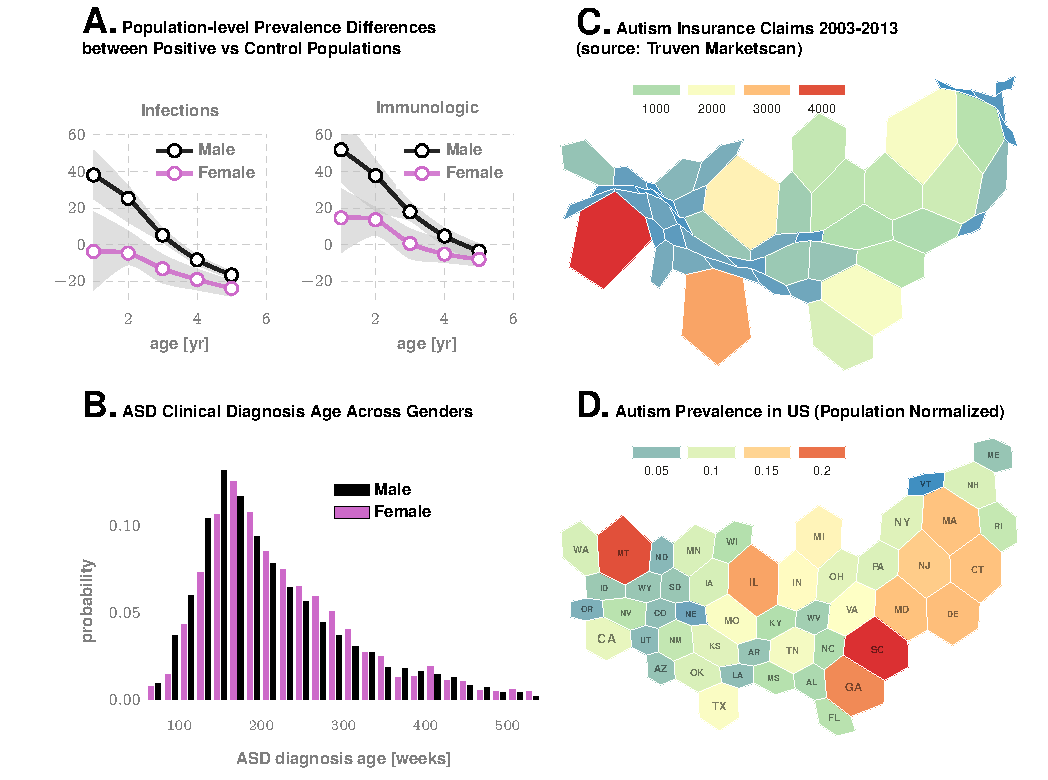
\includegraphics[width=0.9\textwidth]{Figures/External/occur}
  \fi
   
  \captionN{ASD Occurrence Patterns. 
    Panel A illustrates the differential representation of different disease categories in the \treatment and control cohorts, and panel B shows the distribution of the age of  diagnosis for males and females in the Truven dataset. Panel C illustrates the spatial distribution of ASD insurance claims, and panel D shows the same data after population normalization, illustrating the relatively small demographic skew to ASD prevalence within the general population with access to medical insurance, which is consistent with the suggestion that prevalence variation might be linked to regional and socioeconomic disparities in access to services~\cite{jarquin2011racial}.
  }\label{EXT-fig0}
\end{figure}
\else
\refstepcounter{figure}\label{EXT-fig0}
\fi
% ###########################################################
% ###########################################################
% ##########################################
\begin{table*}[!ht]
  \begin{center}
    \captionN{Patient Counts In De-identified Data \& The Fraction of Datasets Excluded By Our Exclusion Criteria$^\star$}\label{tab2}
    \sffamily\small
    \begin{tabular}{L{1.5in}L{.695in}L{.695in}C{.695in}L{.695in}L{.695in}}
      &\multicolumn{2}{c@{\quad}}{Truven}    
      &&                                           
         \multicolumn{2}{c}{UCM} \\\cline{2-3}\cline{5-6}          
      Distinct Patients &\multicolumn{2}{c@{\quad}}{115,805,687}    
      &&                                           
         \multicolumn{2}{c}{69,484} \\\cline{2-3}\cline{5-6}          
      &Male& Female    && Male  &Female      \\
      \hline
      ASD Diagnosis Count$^\dag$ & 12,146 & 3,018& &307& 70 \\\hline
      Control Count$^\dag$ & 2,301,952 & 2,186,468 & & 20,249& 17,386\\\hline
      AUC at 125 weeks & 82.3\% & 82.5\% & &83.1\%& 81.37\%\\\hline
      AUC at 150 weeks & 84.79\% & 85.26\% & &82.15\%& 83.39\%\\\hline
      &&     &  &   &      \\
      \multicolumn{5}{c}{Excluded Fraction of the Data sets}      &      \\
      &&     &  &   &      \\
      \hline
      Positive Category & 0.0002 & 0.0& &0.0160& 0.0 \\\hline
      Control Category & 0.0045 &0.0045 & &0.0413&  0.0476\\\hline

      &&     &  &   &      \\
      \multicolumn{6}{c}{Average Number of Diagnostic Codes In Excluded Patients (corresponding number in included patients)}           \\
      &&     &  &   &      \\
      \hline
      Positive Category & 4.33 (35.93) & 0.0 (36.07)& &2.6 (9.75)& 0.0 (10.18) \\\hline
      Control Category & 1.57 (17.06) & 1.48 (15.96)  & & 2.32 (6.8)& 2.07 (6.79) \\\hline

    \end{tabular}


  \end{center}
  \vskip 1em
  \small
  $^\dag$ Cohort sizes are smaller than the total number of distinct patients due to the following exclusion criteria: 1) At least one code within our complete set of tracked diagnostic codes is present in the patient record, 2) Time-lag between first and last available record for a patient is at least 15 weeks.

  $^\star$ Dataset sizes are after the exclusion criteria are applied
\end{table*}
% ###########################################################
% ###########################################################
\begin{table*}[!t]
  \centering
  
  \captionN{Disease Categories (A few ICD9 codes shown from the complete set of $9,835$ unique ICD9 codes considered. See SI-Table~\ref{SI-tab0} in  Supplementary text for complete list)}\label{EXT-tab0}
  \vskip .5em
  
  \small\color{black!90}
  \begin{tabular}{L{1in}|L{2in} | |L{3in}}\hline
    \bf\sffamily   Category$^\dag$ & \bf\sffamily  Description  & \bf\sffamily  Examples of ICD9$^\star$ Codes \\\hline
    \rowcolor{lightgray!80}ASD$^\star$ & Diagnostic Target & 299 299.0 299.00 299.01 299.9 299.8 299.91 299.90 299.80 299.81 299.1 299.10 299.11\\\hline
    \cellcolor{Red1!70}Immunologic & Diseases related to dys-regulation of the Immune system &580.81 580.89 580.0 580.8 461 461.8 461.0 477.9 477.2 477 477.8\\\hline
    \cellcolor{Red1!70}Infectious & Diseases Caused By Pathogens &487.8 488.12 488.0 488.01 487.0 487.1 488.09 464.4 466 466.11 466.1\\\hline
    \cellcolor{Red1!50}Nutrition &  Symptoms concerning nutrition, metabolism and development   & 783.0 783.21 783.3 783.40 783.42 783.7 783.9\\\hline
    \cellcolor{Red1!50}Mental Disorders & Psychiatric phenotypes other than ASD & 290 -  319 (except 299.x) \\\hline
    \cellcolor{Red1!50}Health Services &Contact With   Health Services and Classification Of Factors Influencing Health Status  & V01.0 V01.1 V01.2 V01.3 V01.4   V09.70 V09.71 V88.02 V88.03 V89.01 V89.02 V89.03 V89.04 V89.05 V89.09 \\\hline
    \cellcolor{IndianRed1!50}Digestive & Diseases Of The Digestive System &540.0 540.1 541.0 542 540 541 543.0 562.03 562.01 562.00 562.10\\\hline
    \cellcolor{IndianRed1!50}Otic & Diseases Of The Ear And Mastoid Process
                                                                &381.51 381.50 381.81 381.89 381.61 381.62 381 381.7 385.82 383.32 380.30\\\hline
    \cellcolor{IndianRed1!50}Musculoskeletal & Congenital musculoskeletal anomalies &756.52 756.53 733.02 733.0 733.09 737.43 737.41 737.20 737.29 737.4 737.2\\\hline
    \cellcolor{IndianRed1!50}Developmental & Congenital  anomalies (Non-overlapping with muskuloskeletal)  &755.55 743.45 743.11 743.10 743.00 743.03 743.44 743.22 743.20 743.21 758.4\\\hline
    \cellcolor{IndianRed1!30}Reproductive & Diseases Of The Genitourinary System   &611.79 611.71 611.89 611.81 676.64 611 676.60 611.6 611.4 611.3 611.2\\\hline
    \cellcolor{IndianRed1!20}Integumentary & Diseases Of Skin And Subcutaneous Tissue &706.0 706.1 704.00 704.02 704.09 680.9 680.1 680.5 680.7 680.6 680\\\hline
    % 
    Ophthalmologic & Disorders Of The Eye And Adnexa &362.8 362.9 362.6 362.1 362.3 362.18 362.17 362.13 362.11 363.33 363.32\\\hline
    Hematologic &  Diseases Of The Blood And Blood-Forming Organs & 286.9 286.6 283.19 283.11 283.9 283.1 284.0 284.09 284 284.01\\\hline
    Metabolic & Metabolic Disorders (Non-overlapping with respiratory, digestive and immunological conditions) &273.4 270 270.3 712.11 712.13 712.12 712.14 712.18 712.30 712.37 712.36\\\hline
    Cardiovascular & Diseases Of Arteries, Arterioles, And Capillaries  &442.89 441.6 442.82 442.83 441.03 441.02 441.00 442 414.11 447.70 447.71\\\hline
    Respiratory & Diseases Of The Respiratory System (non-overlapping with Infectious) &516.31 516.30 516.32 516.35 516.37 516.36 516.8 516.0 277.0 277.00 277.01\\\hline
    Endocrine & Disorders Of Thyroid and other Endocrine Glands &244 244.9 244.2 255.41 255.5 255.4 259.51 255 259.4 255.11 242.2\\\hline
  \end{tabular}
  \vskip 1em
  \small
  $^\dag$ Categories inferred to be   important for risk modulation are proportionately highlighted.\\
  $^\star$ ICD10 codes when present were mapped back to closest ICD9 matches using published General Equivalence Mappings~\cite{GEMS}.
\end{table*}
% ###########################################################
% ###########################################################
% ###########################################################


% ###########################################################
\begin{table*}[t]
  \centering
  
  \captionN{Engineered Features (Total Count: 165)}\label{EXT-tab1}
  \vskip .5em

  \begin{tabular}{L{2.25in}|L{3in}|C{1in}} \hline
    \textbf{Feature Type$^\ddag$}               & \textbf{Description}   & \textbf{No. of Features}   \\\hline
    {[}Disease Category{]}$_{ \ \Delta}$               & Likelihood Defect (See Methods section) & 17   \\\hline
    {[}Disease Category{]}$_{ \ 0}$               & Likelihood of control model (See Methods section) & 17  \\\hline
    {[}Disease Category{]}$_{\textrm{ proportion}}$   & Occurrences in the encoded sequence / length of the sequence         & 17\\\hline
    {[}Disease Category{]}$_{\textrm{ streak}}$      & Maximum Length of adjacent occurrences  of {[}Disease Category{]}    & 51      \\\hline
    {[}Disease Category{]}$_\textrm{ prevalence}$   &  Maximum, mean  and variance of Occurrences in the encoded sequence / Total Number of diagnostic codes in the mapped sequence   & 51      \\\hline
    Feature Mean, Feature Variance, Feature Maximum for difference of control and case models                 & Mean, Variance, Maximum of the {[}Disease Category{]}$_{ \ \Delta}$ values   & 3     \\\hline
    Feature Mean, Feature Variance, Feature Maximum for control models               & Mean, Variance, Maximum of the {[}Disease Category{]}$_{\ 0}$ values   & 3     \\\hline
    Streak      & Maximum, mean  and variance of the length of adjacent occurrences  of {[}Disease Category{]}    & 3      \\\hline
    Intermission& Maximum, mean  and variance of the length of adjacent empty weeks     & 3    \\\hline
  \end{tabular}
  \vskip 1em
  \small
  $^\ddag$ Disease categories are described in Table~\ref{EXT-tab0}
\end{table*}
% ###########################################################
% ###########################################################
% ###########################################################

% ###########################################################
% ###########################################################
\ifFIGS
\begin{figure*}[!t]
  \tikzexternalenable
  \tikzsetnextfilename{perfA}

  \centering  
   
  \def\DATA{../../data_revision}
  \iftikzX
  \begin{tikzpicture}[font=\bf\sffamily\fontsize{8}{10}\selectfont]
\def\TEXTCOL{gray}
    % \tikzset{
    %     hatch distance/.store in=\hatchdistance,
    %     hatch distance=20pt,
    %     hatch thickness/.store in=\hatchthickness,
    %     hatch thickness=2pt
    % }

% defining the new dimensions and parameters
\newlength{\hatchspread}
\newlength{\hatchthickness}
\newlength{\hatchshift}
\newcommand{\hatchcolor}{}
% declaring the keys in tikz
\makeatletter
\tikzset{hatchspread/.code={\setlength{\hatchspread}{#1}},
         hatchthickness/.code={\setlength{\hatchthickness}{#1}},
         hatchshift/.code={\setlength{\hatchshift}{#1}},% must be >= 0
         hatchcolor/.code={\renewcommand{\hatchcolor}{#1}}}
% setting the default values
\tikzset{hatchspread=3pt,
         hatchthickness=0.4pt,
         hatchshift=0pt,% must be >= 0
         hatchcolor=black}
% declaring the pattern
\pgfdeclarepatternformonly[\hatchspread,\hatchthickness,\hatchshift,\hatchcolor]% variables
   {custom north west lines}% name
   {\pgfqpoint{\dimexpr-2\hatchthickness}{\dimexpr-2\hatchthickness}}% lower left corner
   {\pgfqpoint{\dimexpr\hatchspread+2\hatchthickness}{\dimexpr\hatchspread+2\hatchthickness}}% upper right corner
   {\pgfqpoint{\dimexpr\hatchspread}{\dimexpr\hatchspread}}% tile size
   {% shape description
    \pgfsetlinewidth{\hatchthickness}
    \pgfpathmoveto{\pgfqpoint{0pt}{\dimexpr\hatchspread+\hatchshift}}
    \pgfpathlineto{\pgfqpoint{\dimexpr\hatchspread+0.15pt+\hatchshift}{-0.15pt}}
    \ifdim \hatchshift > 0pt
      \pgfpathmoveto{\pgfqpoint{0pt}{\hatchshift}}
      \pgfpathlineto{\pgfqpoint{\dimexpr0.15pt+\hatchshift}{-0.15pt}}
    \fi
    \pgfsetstrokecolor{\hatchcolor}
%    \pgfsetdash{{1pt}{1pt}}{0pt}% dashing cannot work correctly in all situation this way
    \pgfusepath{stroke}
   }
 \makeatother


%     \makeatletter
%     \pgfdeclarepatternformonly[\hatchdistance,\hatchthickness]{flexible hatch}
%     {\pgfqpoint{0pt}{0pt}}
%     {\pgfqpoint{\hatchdistance}{\hatchdistance}}
%     {\pgfpoint{\hatchdistance-1pt}{\hatchdistance-1pt}}%
%     {
%         \pgfsetcolor{\tikz@pattern@color}
%         \pgfsetlinewidth{\hatchthickness}
%         \pgfpathmoveto{\pgfqpoint{0pt}{0pt}}
%         \pgfpathlineto{\pgfqpoint{\hatchdistance}{\hatchdistance}}
%         \pgfusepath{stroke}
%     }
%     \makeatother
% \pgfdeclarepatternformonly{north east lines wide}%
%    {\pgfqpoint{-1pt}{-1pt}}%
%    {\pgfqpoint{10pt}{10pt}}%
%    {\pgfqpoint{9pt}{9pt}}%
%    {
%      \pgfsetlinewidth{0.4pt}
%      \pgfpathmoveto{\pgfqpoint{0pt}{0pt}}
%      \pgfpathlineto{\pgfqpoint{9.1pt}{9.1pt}}
%      \pgfusepath{stroke}
%     }


  \def\WDT{4.75in} 
  \def\WDTA{2in}    

  \def\datafile{../../data_revision/figfiles/AUC.csv}
  \def\datafileimp{../../data_revision/figfiles/AUC_imputed.csv}
 % \def\CHLM{Figures/augmented_M_fips_auc_rainbow}
 % \def\CHLF{Figures/augmented_F_fips_auc_rainbow}

  \def\CHLM{../../data_revision/figfiles/augmented_M_fips_auc_rainbow0}
  \def\CHLF{../../data_revision/figfiles/augmented_F_fips_auc_rainbow0}
  % \def\CHLM{Figures/augmented_M_fips_auc_Spectral_r0}
  % \def\CHLF{Figures/augmented_F_fips_auc_Spectral_r0}
  % \def\CHLM{Figures/augmented_M_fips_auc_Purples0}
  % \def\CHLF{Figures/augmented_F_fips_auc_Purples0}

  \def\ROCF{../../data_revision/figfiles/ROC_F_s.csv}
  \def\ROCM{../../data_revision/figfiles/ROC_M_s.csv}
  \def\IMP{../../data_revision/figfiles/importance20.csv}
  \def\IMP{../../data_revision/figfiles/importance15.csv}
  \def\INTF{Figures/intf.dat}

  \def\HGT{1.30in}
  \def\WDT{6in}
  \def\WDTC{4in}
  \def\WDTR{1.9in}
  \def\WDTH{1.7in}
  
  \node[] (A) at (0,0) {};
  \node [anchor=north] (M) at (A.south) {\includegraphics[width=\WDTC]{\CHLM}};
  \node [anchor=north] (F) at ([yshift=-0.8in]M.south) {\includegraphics[width=\WDTC]{\CHLF}};
  
  % \begin{axis}[legend cell align=left,text=\TEXTCOL,
  %   legend style={text=black,anchor=east,at={(0.32,0.4)},inner sep=3pt,draw=none,fill=lightgray!10,fill opacity=.35,align=right,text opacity=1},
  %   name=E,
  %   at=(F.south west),
  %   xshift=0.6in,
  %   yshift=-0.7in,
  %   anchor=north west,
  %   width=\WDT,
  %   height=\HGT,
  %   ybar,
  %   bar width=4pt,
  %   xmin=.6,
  %   xmax=1,
  %   scale only axis=true, 
  %   axis on top=false,
  %   % axis background/.style={
  %   % shade,top color=transparent!15,bottom color=transparent!10},
  %   axis line style={lightgray!2, thin},
  %   grid,
  %   grid style={dashed,opacity=.95,thin,black!10},
  %   % xticklabel style={xshift=0.05in,yshift=-.05in},
  %   % xlabel style={xshift=-.075in,yshift=.05in,text=black},
  %   ylabel style={align=center,,text=black,anchor=center,
  %     yshift=-.1in,xshift=-.1in,font=\bf\sffamily\fontsize{7}{8}\selectfont,text=\TEXTCOL},
  %   % tickpos=left,
  %   ytick align=outside,
  %   xtick align=outside,
  %   major tick length=0pt,
  %   scaled y ticks = false,
  %   y tick label style={/pgf/number format/fixed,
  %     /pgf/number format/1000 sep = \thinspace % Optional if you want to replace comma as the 1000 separator 
  %   },
  %   ylabel={probability},
  %   ytick={0,0.02,0.04,0.06,0.08},
  %   ]
  %   \addplot [draw=none, thin, fill=\FXCOL,,fill opacity=1,, area legend]table [col sep=comma,x=AUC,y=F, area legend] {\datafileimp};
  %   \addlegendentry{AUC (Female)};
  %   \addplot [draw=none, thin, fill=\MXCOL,fill opacity=1, area legend] table [col sep=comma,x=AUC,y=M, area legend] {\datafileimp};
  %   \addlegendentry{AUC (Male)};
  %   % \draw[very thick,Red2] (axis cs:0.677,\pgfkeysvalueof{/pgfplots/ymin}) -- (axis cs:0.677,\pgfkeysvalueof{/pgfplots/ymax}) node [midway,right,fill=white,fill opacity=.9,text opacity=1,inner sep=2pt,pos=0.2,font=\sffamily\fontsize{6}{6}\selectfont] {0.677};
  %   % \draw[very thick,Red2] (axis cs:0.73,\pgfkeysvalueof{/pgfplots/ymin}) -- (axis cs:0.73,\pgfkeysvalueof{/pgfplots/ymax}) node [midway,right,fill=white,fill opacity=.9,text opacity=1,inner sep=2pt,pos=0.2,font=\sffamily\fontsize{6}{6}\selectfont] {0.73};
  % \end{axis}
  
  \node [anchor=north east, align=left,align=left] (B) at ([xshift=-0.35in,yshift=0.1in]M.north west) {
    \begin{tikzpicture}[anchor=center]
    \begin{axis}[legend cell align=left,text=\TEXTCOL, legend style={text=black,anchor=east,at={(1,0.12)},inner sep=1pt,draw=none,fill=gray!19,fill opacity=.85,align=right,text opacity=1,font=\bf\sffamily\fontsize{7}{8}\selectfont},
    name=K,
    clip=false,
    %at=(CC.center),
    xshift=-0in,
    yshift=-.25in,
    anchor=center,
    width=\WDTR,
    height=\WDTH,
    scale only axis=true,
    enlargelimits=false,
    axis on top=false,
     axis background/.style={
     shade,top color=transparent!0,bottom color=transparent!15},
    axis line style={black!2, very thick},
    grid,
    grid style={opacity=.9,thin,black!20},
    % xticklabel style={xshift=0.05in,yshift=-.05in},
    xlabel style={yshift=.05in,text=\TEXTCOL},
    ylabel style={align=center,,text=\TEXTCOL,anchor=center,
      yshift=-.175in},
    % tickpos=left,
    ytick align=outside,
    xtick align=outside,
    major tick length=0pt,
    scaled y ticks = false,
    y tick label style={/pgf/number format/fixed,
      /pgf/number format/1000 sep = \thinspace % Optional if you want to replace comma as the 1000 separator 
    },
    ylabel={TPR},xlabel={FPR},
    xmin=-0.05,
    ymax=1.02,
    extra x ticks={1},extra x tick labels={1}]
%
    \def\LCOL{Red1}
        \addplot [name path=a,smooth,draw=\FXCOL, ultra thick, fill=none,, pattern color=\FXCOL,pattern=custom north west lines,hatchspread=6pt,hatchthickness=3pt,fill opacity=.35,hatchcolor=Orchid3!60]table [col sep=comma,x=fpr ,y=tpr] {\ROCF};
          \addlegendentry{Female (AUC 85.2\%)}
  \addplot [smooth,draw=\MXCOL, ultra thick, fill=none,fill opacity=.5,]table [col sep=comma,x=fpr ,y=tpr] {\ROCM};
    \addlegendentry{Male (AUC 84.7\%)} 


\draw[name path=b,smooth,draw=\LCOL,,,very thick] (axis cs:0.05,0) -- (axis cs:0.05,\pgfkeysvalueof{/pgfplots/ymax})
      %\addplot [name path=b,smooth,draw=\LCOL,,,very thick]table [col sep=comma,x=fpr ,y=tpr] {\INTF} 
node [fill=white,midway,sloped,above,right,pos=.725,yshift=-.165in,text=\LCOL,align=center,font=\bf\sffamily\fontsize{7}{8}\selectfont] {specificity \\95.0\%};
      %\draw[Red1,name path=b,] (axis cs:0.05,0) -- (axis cs:0.05,1);
      \fill [name intersections={of=a and b},Red1] (intersection-1) circle (2pt)coordinate (c) ;


      \draw [\LCOL,very thick] (c) -- ($(axis cs:\pgfkeysvalueof{/pgfplots/xmin},0)!(c)!(axis cs:\pgfkeysvalueof{/pgfplots/xmin},1)$) ;
      \draw [\LCOL,very thick] (c) -- ($(axis cs:1,0)!(c)!(axis cs:1,1)$)node [font=\bf\sffamily\fontsize{7}{8}\selectfont,fill=lightgray!50,midway,below,pos=.7,yshift=-.1in,text=\LCOL] {sensitivity: 51.8\%\\PPV (Male): 15.8\%\\PPV (Female): 18.8\%};
      % \draw [black,name path=d] (axis cs:0,0.38) -- (axis cs:1,.38)node [midway,below,pos=.65] {M-CHAT/F 38.8\%};
      % \fill [name intersections={of=d and b},black] (intersection-1) circle (2pt)coordinate (dd) ;
      %\draw[ultra thin,dashed,black] (c) -- (axis cs:1,.5175);
    \end{axis}
    \end{tikzpicture} 
  };
%
  \node [anchor=north east,align=left] (R) at ([xshift=-1.55in,yshift=1in]F.north west) {

\begin{axis}[legend cell align=left,legend style={anchor=east,at={(.9,0.1)},inner sep=3pt,draw=none,fill=white,fill opacity=.85,align=right,text opacity=1,font=\bf\sffamily\fontsize{8}{9}\selectfont},axis line style={lightgray, opacity=0, thin},%
enlargelimits=true,
%grid,
xshift=.1in,
anchor=north west,
  height=4in,
width=2.15in,
    xbar, 
    ytick=data,% crucial line for the xticklabels directive 
    ymin=0, 
    yticklabels from table={\IMP}{feature},
        yticklabel style={font=\bf\sffamily\fontsize{7}{7}\selectfont,align=right,rotate=0, text width=1.1in, anchor=east, yshift=0in,xshift=-.045in,text=\TEXTCOL},
major tick length=0pt,
xticklabel style={font=\bf\sffamily\fontsize{7}{7}\selectfont,text=\TEXTCOL},
grid,
grid style={lightgray, opacity=.7},
axis on top=false, bar width=4.2pt,xlabel={importance},xlabel style={yshift=0.05in,text=\TEXTCOL},
enlarge y limits=0.03,
] 

\addplot[opacity=1,fill=\MXCOL, area legend] table [ 
    y expr=\coordindex,
    x=M
] {\IMP};   
\addlegendentry{Male}
\addplot[opacity=1,fill=\FXCOL, area legend] table [ 
    y expr=\coordindex,
    x=F
] {\IMP};   
\addlegendentry{Female}

\end{axis} 

  };

  \node[anchor=south west,align=left] (LA) at ([xshift=.2in,yshift=0in]M.north west) {{\LARGE C.} AUC Spatial Variation (Males)   };
  \node[anchor=south west,align=left] (LB) at ([xshift=.2in,yshift=0in]F.north west) {{\LARGE D.} AUC Spatial Variation (Females)   };
  %\node[anchor=south west,align=left] (LC) at ([xshift=0in,yshift=.1in]$(LA.west)!(E.north west)!(LB.west)$) {{\LARGE C.} AUC Distribution over US Counties};
  \node[anchor=north west,align=left] (LD) at ([xshift=-0in,yshift=0in]$(B.west)!(LA.north)!(B.north west)$) {{\LARGE A.} ROC Curves at $150$ weeks  };

  \node[anchor=south west,align=left] (LR) at ([xshift=-0in,yshift=0.05in]$(LD.north west)!(R.north)!(LD.south west)$) {{\LARGE B.} Top 15  Phenotype-specific Features };

\end{tikzpicture}

  \else
  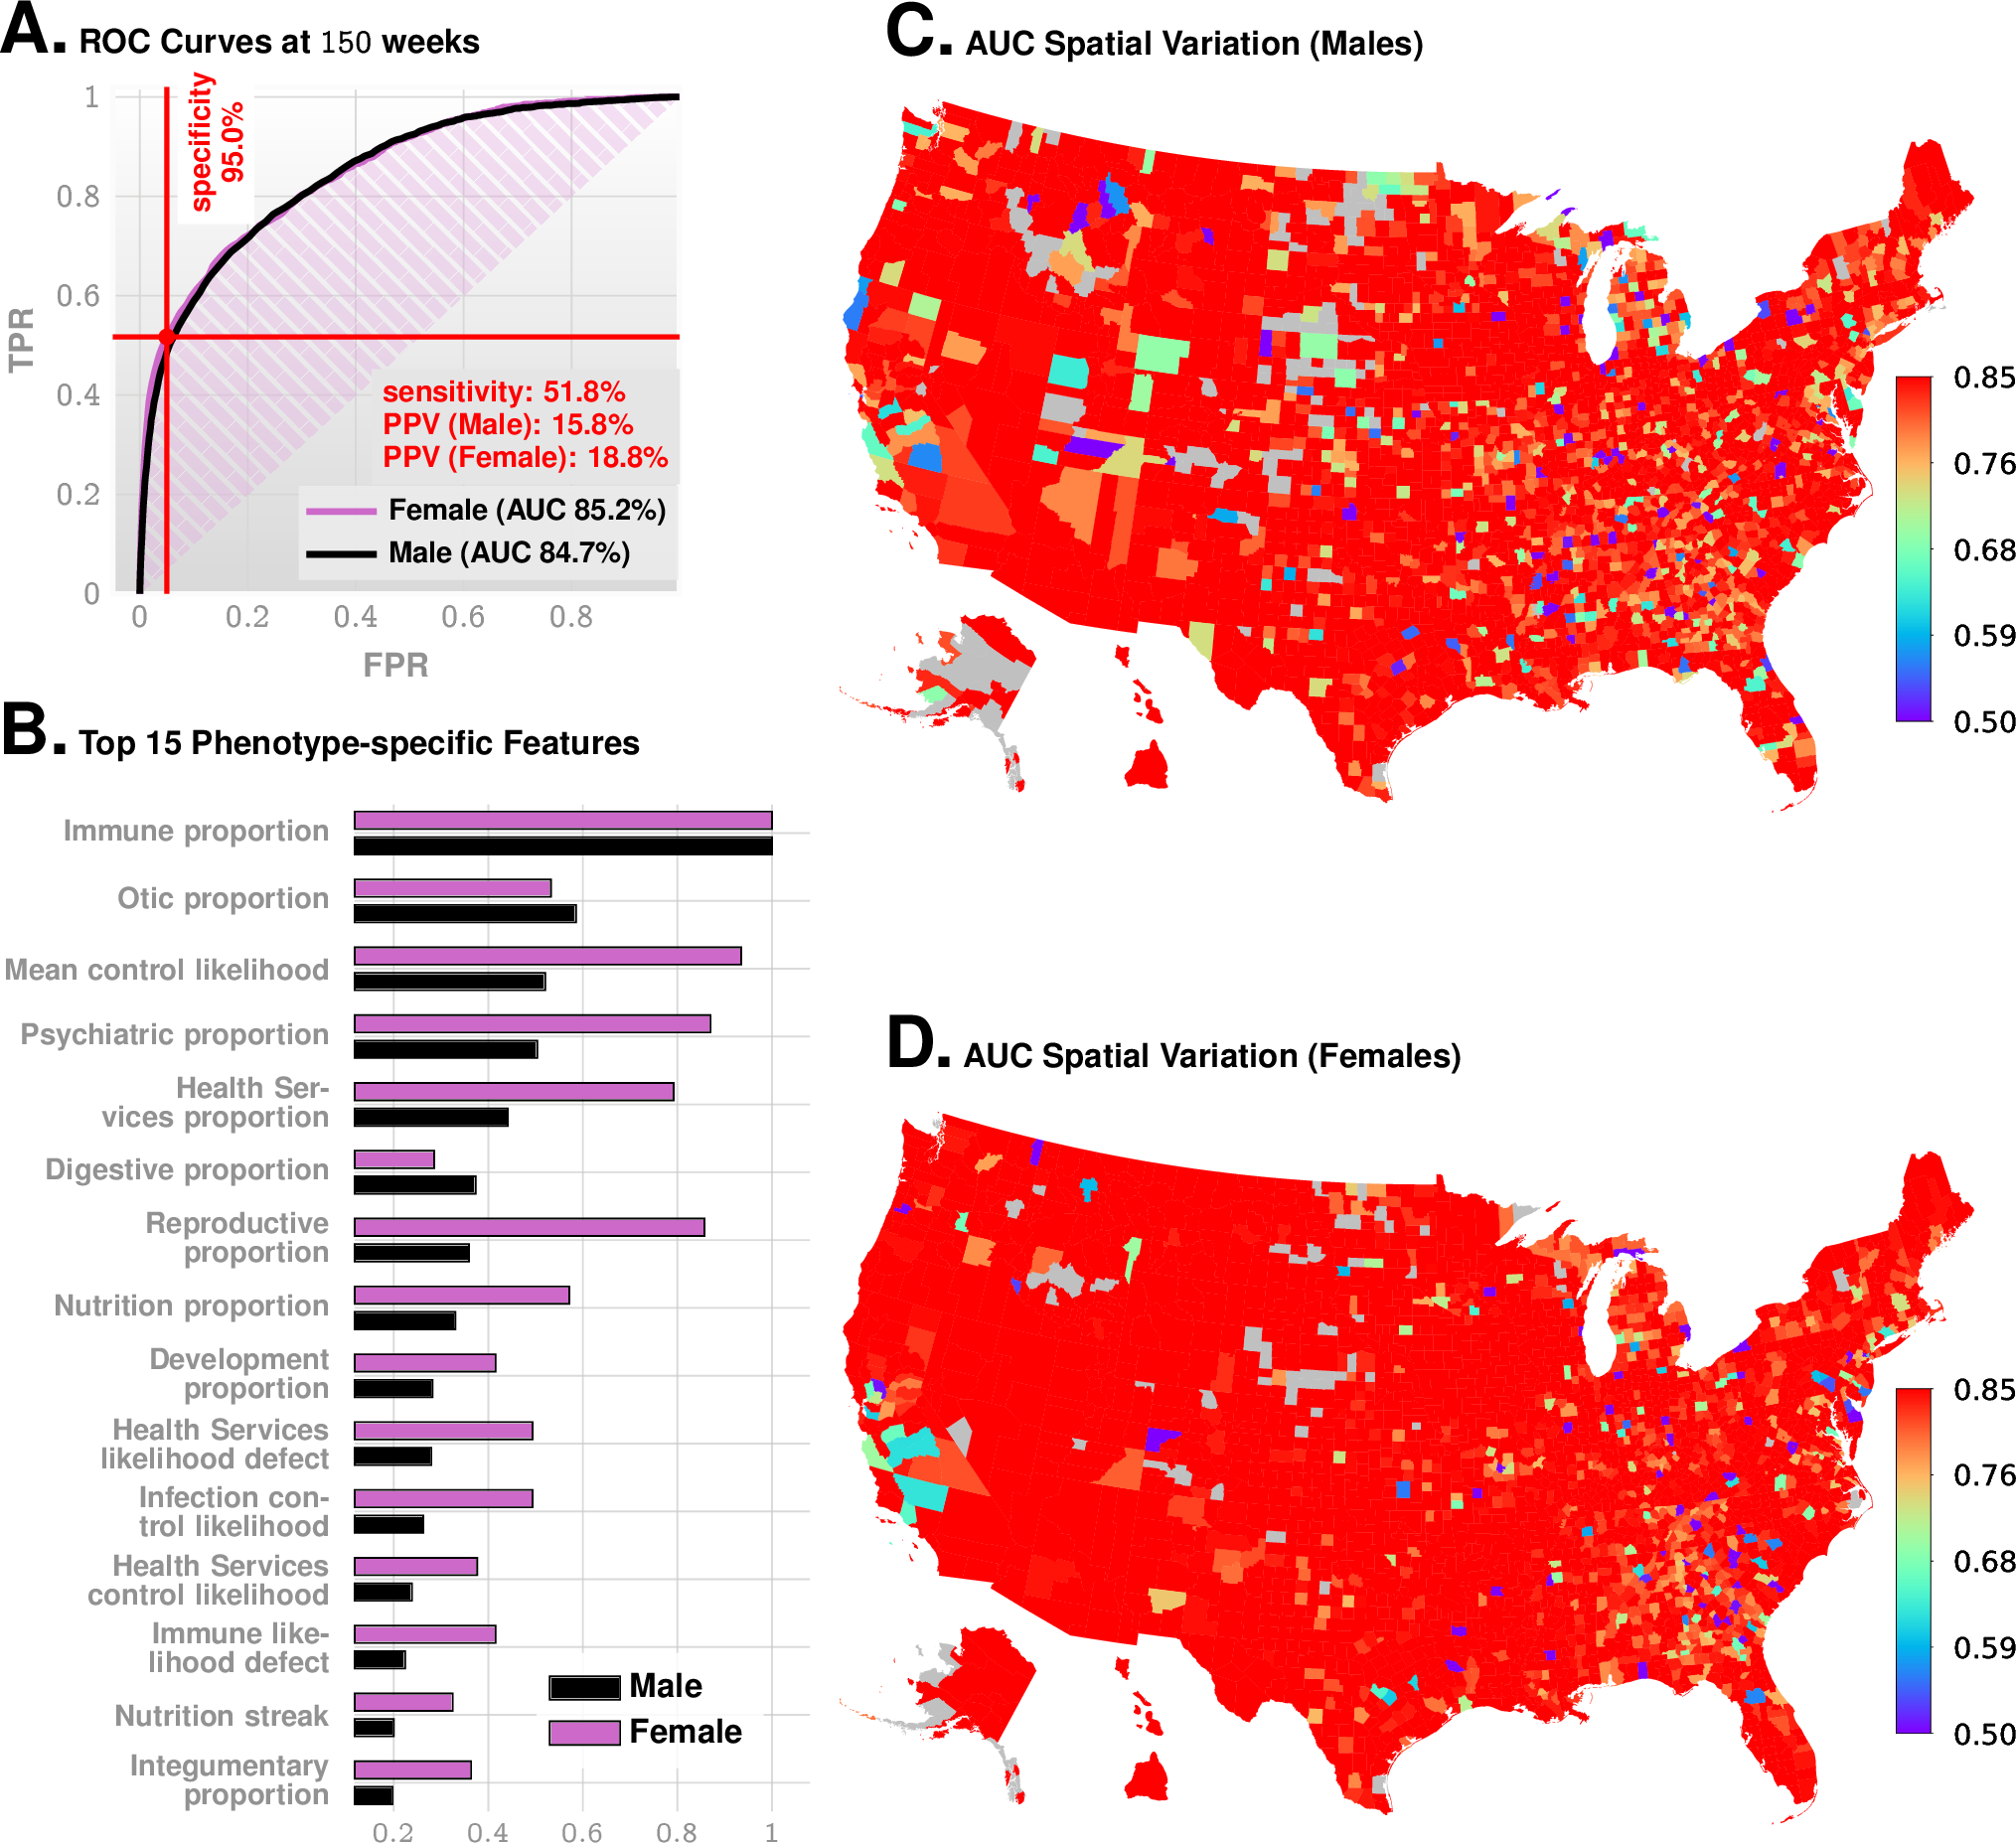
\includegraphics[width=0.85\textwidth]{Figures/External/perfA.pdf}
  \fi

  \captionN{Predictive Performance. Panel %C shows the distribution of the AUC, and panel
    A shows the ROC curves for males and females. Panel B shows the feature importance inferred by our prediction pipeline. The detailed description of the features is given in Table~\ref{EXT-tab0}. The most import feature is related to immunologic disorders, and we note that in addition to features related to individual disease categories, we also have the mean control likelihood (rank 3), which may be interpreted as the average likelihood of the diagnostic patterns correspond to the control category as opposed to the \treatment category. Panels C and D show the spatial variation in the achieved predictive performance at 150 weeks, measured by AUC, for males and females, respectively. Gray areas lack data on either positive or negative cases. These county-specific AUC plots show that the performance of the algorithm has  relatively weak geospatial dependence, which is important in the light of current uneven distribution of diagnostic resources.
  }\label{fig1}
\end{figure*}
\else
\refstepcounter{figure}\label{fig1}
\fi
% ###########################################################
% ###########################################################
% ###########################################################
% ###########################################################
\ifFIGS
\begin{figure*}[!ht]
  \tikzexternalenable
  \tikzsetnextfilename{perfB}
  
  \centering 
  \def\DATA{../../data_revision}
  \iftikzX
  

\pgfplotsset{
    discard if/.style 2 args={
        x filter/.append code={
            \edef\tempa{\thisrow{#1}}
            \edef\tempb{#2}
            \ifx\tempa\tempb
                \def\pgfmathresult{inf}
            \fi
        }
    },
    discard if not/.style 2 args={
        x filter/.append code={
            \edef\tempa{\thisrow{#1}}
            \edef\tempb{#2}
            \ifx\tempa\tempb
            \else
                \def\pgfmathresult{inf}
            \fi
        }
    }
  }

  \begin{tikzpicture}[font=\bf\sffamily\fontsize{8}{10}\selectfont]
\def\TEXTCOL{gray}
    \tikzset{
        hatch distance/.store in=\hatchdistance,
        hatch distance=20pt,
        hatch thickness/.store in=\hatchthickness,
        hatch thickness=2pt
    }

%     \makeatletter
%     \pgfdeclarepatternformonly[\hatchdistance,\hatchthickness]{flexible hatch}
%     {\pgfqpoint{0pt}{0pt}}
%     {\pgfqpoint{\hatchdistance}{\hatchdistance}}
%     {\pgfpoint{\hatchdistance-1pt}{\hatchdistance-1pt}}%
%     {
%         \pgfsetcolor{\tikz@pattern@color}
%         \pgfsetlinewidth{\hatchthickness}
%         \pgfpathmoveto{\pgfqpoint{0pt}{0pt}}
%         \pgfpathlineto{\pgfqpoint{\hatchdistance}{\hatchdistance}}
%         \pgfusepath{stroke}
%     }
%     \makeatother
% \pgfdeclarepatternformonly{north east lines wide}%
%    {\pgfqpoint{-1pt}{-1pt}}%
%    {\pgfqpoint{10pt}{10pt}}%
%    {\pgfqpoint{9pt}{9pt}}%
%    {
%      \pgfsetlinewidth{0.4pt}
%      \pgfpathmoveto{\pgfqpoint{0pt}{0pt}}
%      \pgfpathlineto{\pgfqpoint{9.1pt}{9.1pt}}
%      \pgfusepath{stroke}
%     }


  \def\WDT{4.75in} 
  \def\WDTA{2in} 

  \def\datafile{../../data_latest/figfiles/model_complexity.csv}
  \def\riskfile{\DATA/figfiles/risk.csv}
  \def\sampleimg{\DATA/figfiles/sample.pdf}
  \def\sampledat{\DATA/figfiles/sampledat.csv}
  \def\auctime{\DATA/figfiles/auc_time.csv}
  \def\auctimeV{\DATA/figfiles/Vauc_time.csv}
  \def\randomsamples{\DATA/figfiles/cfbd_auctime.csv}

  
  \def\horzm{../../perturbation_browser/ntb/male_horizon.csv}
  \def\horzmt{../../perturbation_browser/ntb/male_horizon_T.csv}
 \def\horzf{../../perturbation_browser/ntb/female_horizon.csv}
  \def\horzft{../../perturbation_browser/ntb/female_horizon_T.csv}
  \def\perturbneg{../../perturbation_browser/ntb/perturb_neg.csv}
  \def\track{../../perturbation_browser/ntb/track.csv}

  \def\PNEGA{A020571551}
  \def\PNEGB{A005421148}
  \def\PNEGC{A033768823}
  \def\PPOSA{A006621658}
  \def\PPOSB{A002483419}
  \def\PPOSC{A069615715}

  \def\HGT{1.6in}
  \def\WDT{3.5in}
  \def\WDTC{4in}
  \def\WDTR{1.9in}
  \def\WDTH{1.70in}

  \def\AXISCOL{white}
\def\BANDCOL{lightgray}
\def\PLOTCOLA{black}
\def\PLOTCOLB{\MXCOL}
\def\PLOTCOLBu{\MXCOL}
\def\PLOTCOLC{black}
\def\PLOTCOLD{\FXCOL}
\def\FNCOLB{SeaGreen2}
\def\PLOTCOLDu{\FXCOL}
\def\WDTa{1.85in}
\def\HGTa{2.6in}
\def\HGTaa{3.3in}
\def\WDTb{1in}
\def\HGTb{1.575in}

\def\SCALE{1.5}
\def\SCALEA{1.15}
\def\SCALEB{1.15}
\def\OPC{.75}
\def\OPCB{.85}
\def\BWIDTH{4pt}
\def\LWDT{0.5mm}
  \node[] (A0) at (0,0) {};

  \node[anchor=center] (N) at ([yshift=1in]A0.south)
  {
    \begin{tikzpicture}
       \begin{axis} [,legend cell align={left},
      legend style={anchor=east,at={(0,1.05)},
        inner sep=3pt,
        draw=none,
        fill=white,fill opacity=.85,
        align=left,anchor=west,
        text opacity=1,
        font=\bf\sffamily\fontsize{8}{9}\selectfont,text=black},
      grid style={thick,dashed, gray!40},
      grid,
    enlargelimits=true,scale only axis=true,scaled x ticks = false,scaled y ticks = false,
     height=\HGTa,
    width=\WDTa,
    enlarge x limits=0.07,axis line style={\AXISCOL, opacity=1,ultra  thick, rounded corners=0pt}, y tick label style={/pgf/number format/fixed,/pgf/number format/precision=3,/pgf/number format/fixed zerofill,
     /pgf/number format/1000 sep = %\thinspace % Optional if you want to replace comma as the 1000 separator 
      },
      major tick length=0pt,legend columns=2, legend style={,xshift=-.5in,yshift=.2in},
      yshift=-.75in,text=\TEXTCOL,xlabel={age [weeks]},xlabel style={yshift=0.025in},ylabel
      style={xshift=-0.1in},ylabel={AUC},
      grid style={thick,dashed, gray!40},
      ymax=0.9]

      
    \addplot[forget plot,smooth, draw=none,,name path=AA]table[col sep=comma,x=week, y=ub, discard if not={gender}{M}, discard if not={dataset}{UCM}]
    {\randomsamples};
    \addplot[forget plot,smooth,  draw=none,,name path=BB]table[col sep=comma,x=week, y=lb, discard if not={gender}{M}, discard if not={dataset}{UCM}]
    {\randomsamples};
    \addplot[forget plot,\MXCOL,opacity=.175] fill between[of=AA and BB];
    
      
    \addplot[forget plot,smooth, draw=none,,name path=AA]table[col sep=comma,x=week, y=ub, discard if not={gender}{F}, discard if not={dataset}{UCM}]
    {\randomsamples};
    \addplot[forget plot,smooth,  draw=none,,name path=BB]table[col sep=comma,x=week, y=lb, discard if not={gender}{F}, discard if not={dataset}{UCM}]
    {\randomsamples};
    \addplot[forget plot,\FXCOL,opacity=.175] fill between[of=AA and BB];
    
    
 \addplot[forget plot,smooth, draw=none,,name path=AA]table[col sep=comma,x=week, y=ub, discard if not={gender}{F}, discard if not={dataset}{Truven}]
    {\randomsamples};
    \addplot[forget plot,smooth,  draw=none,,name path=BB]table[col sep=comma,x=week, y=lb, discard if not={gender}{F}, discard if not={dataset}{Truven}]
    {\randomsamples};
    \addplot[forget plot,\MNCOL,opacity=.175] fill between[of=AA and BB];
    

    
 \addplot[forget plot,smooth, draw=none,,name path=AA]table[col sep=comma,x=week, y=ub, discard if not={gender}{M}, discard if not={dataset}{Truven}]
    {\randomsamples};
    \addplot[forget plot,smooth,  draw=none,,name path=BB]table[col sep=comma,x=week, y=lb, discard if not={gender}{M}, discard if not={dataset}{Truven}]
    {\randomsamples};
    \addplot[forget plot,\FNCOL,opacity=.1750] fill between[of=AA and BB];
    

      \end{axis}

   \begin{axis} [,legend cell align={left},
      legend style={anchor=east,at={(0,1.05)},
        inner sep=3pt,
        draw=none,
        fill=white,fill opacity=.85,
        align=left,anchor=west,
        text opacity=1,
        font=\bf\sffamily\fontsize{8}{9}\selectfont,text=black},
      grid style={thick,dashed, gray!40},
      grid,
    enlargelimits=true,scale only axis=true,scaled x ticks = false,scaled y ticks = false,
     height=\HGTa,
    width=\WDTa,
    enlarge x limits=0.07,axis line style={\AXISCOL, opacity=1,ultra  thick, rounded corners=0pt}, y tick label style={/pgf/number format/fixed,/pgf/number format/precision=3,/pgf/number format/fixed zerofill,
     /pgf/number format/1000 sep = %\thinspace % Optional if you want to replace comma as the 1000 separator 
      },
      major tick length=0pt,legend columns=2, legend style={,xshift=-.5in,yshift=.2in},
      yshift=-.75in,text=\TEXTCOL,xlabel={age [weeks]},xlabel style={yshift=0.025in},ylabel
      style={xshift=-0.1in},ylabel={AUC},
      grid style={thick,dashed, gray!40},
      ymax=0.9]
      
        \draw [draw=none,ultra thick,opacity=.3,postaction={
         pattern=flexible hatch,
        hatch distance=7pt,
        hatch thickness=2pt,
        draw=none,
        opacity=.5,
        pattern color=lightgray, %ultra thick,
     },] (axis cs:130,\pgfkeysvalueof{/pgfplots/ymin}) -- (axis cs:130,\pgfkeysvalueof{/pgfplots/ymax}) -- (axis cs:105,\pgfkeysvalueof{/pgfplots/ymax}) -- (axis cs:105,\pgfkeysvalueof{/pgfplots/ymin}) --cycle;

    \addplot[ smooth,  line width=\LWDT, \PLOTCOLB,mark=*, opacity=\OPC,
    mark options={%
      scale=\SCALEB,draw=\PLOTCOLB,  thick, fill=\PLOTCOLB,  opacity=\OPC,
    },]table[col sep=comma,x=week, y=v, discard if not={gender}{M}, discard if not={dataset}{Truven}]
    {\randomsamples};
    \addlegendentry{Males (Truven)}


    %
    \addplot[ smooth,  line width=\LWDT, \PLOTCOLBu,mark=square*, opacity=.5,
    mark options={%
      scale=\SCALEA,draw=\PLOTCOLBu,  thick, fill=\PLOTCOLBu,  opacity=.5,
    },]table[col sep=comma,x=week, y=v, discard if not={gender}{M}, discard if not={dataset}{UCM}]    {\randomsamples};
    \addlegendentry{Males (UCM)}





    
    \addplot[ smooth,  line width=\LWDT, \PLOTCOLD,mark=*, opacity=\OPCB,
    mark options={%
      scale=\SCALEB,draw=\PLOTCOLD,  thick, fill=\PLOTCOLD,  opacity=\OPCB,
    },]table[col sep=comma,x=week, y=v, discard if not={gender}{F}, discard if not={dataset}{Truven}]    {\randomsamples};
    \addlegendentry{Females (Truven)}
%
%
    \addplot[ smooth,  line width=\LWDT, \PLOTCOLDu,mark=square*, opacity=.5,
    mark options={%
      scale=\SCALEA,draw=\PLOTCOLDu,  thick, fill=\PLOTCOLDu,  opacity=.5,
    },]table[col sep=comma,x=week, y=v, discard if not={gender}{F}, discard if not={dataset}{UCM}]    {\randomsamples};
    \addlegendentry{Females (UCM)}



    

  \end{axis}



\end{tikzpicture}
  };

  
  \node[anchor=north west] (A) at ([xshift=0in,yshift=-.2in]N.north east) {
    \begin{tikzpicture}[anchor=center]
  \begin{groupplot}[group style={group name=A,group size= 2 by 1,horizontal sep=.5in},legend style={anchor=east,at={(.5,1.1)},/tikz/every even column/.append style={column sep=1.5in},legend cell align={left},inner sep=3pt,draw=none,fill=white,fill opacity=.85,align=right,text opacity=1,font=\bf\sffamily\fontsize{8}{9}\selectfont},axis line style={lightgray, opacity=0, thin},%
    enlargelimits=true,
     width=\HGT,
    height=\HGTaa,
     enlarge y limits=0.03,
    ] 
    \nextgroupplot[xbar,bar width=\BWIDTH,    
ytick=data,% crucial line for the xticklabels directive 
    ymin=0, 
    yticklabels from table={\datafile}{feature},
    yticklabel style={font=\bf\sffamily\fontsize{7}{7}\selectfont,align=right,rotate=0, 
text width=1.1in, anchor=east, yshift=0in,xshift=-.045in,text=\TEXTCOL},
    major tick length=0pt,
    yticklabel style={font=\bf\sffamily\fontsize{7}{7}\selectfont,text=\TEXTCOL},
    %grid,
    grid style={lightgray, opacity=.7},
    axis on top=false, 
    xlabel={},
    ylabel style={yshift=-1.25in,text=\TEXTCOL},,ylabel style={yshift=-.15in},
    ylabel={disease groups}]
    \addplot[opacity=1,fill=\MNCOL, area legend] table [ 
    y expr=\coordindex,
    x=NEGM
    ] {\datafile};   
    \addlegendentry{Male Control}
    \addplot[opacity=1,fill=\MXCOL, area legend] table [ 
    y expr=\coordindex,
    x=POSM
    ] {\datafile};   
    \addlegendentry{Male Positive}

    \nextgroupplot[xbar,bar width=\BWIDTH,    ytick=data,% crucial line for the xticklabels directive 
    ymin=0, 
    yticklabels from table={\datafile}{feature},
    yticklabel style={font=\bf\sffamily\fontsize{7}{7}\selectfont,align=right,rotate=0, 
text width=1.1in, anchor=east, yshift=0in,xshift=-.045in,text=\TEXTCOL},
    major tick length=0pt,
    yticklabel style={font=\bf\sffamily\fontsize{7}{7}\selectfont,text=\TEXTCOL},
    %grid,
    grid style={lightgray, opacity=.7},
    axis on top=false, 
    xlabel={model complexity (no. of states)},
    ylabel style={yshift=-0.69in,text=\TEXTCOL},yticklabels=\empty,xlabel style={text=\TEXTCOL,xshift=-.7in,yshift=.05in},]
    \addplot[opacity=1,fill=\FNCOLB, area legend] table [ 
    y expr=\coordindex,
    x=NEGF
    ] {\datafile};   
    \addlegendentry{Female Control}
    \addplot[opacity=1,fill=\FXCOL, area legend] table [ 
    y expr=\coordindex,
    x=POSF
    ] {\datafile};   
    \addlegendentry{Female Positive}
  \end{groupplot}
\end{tikzpicture}
};




\node[anchor=north west] (B) at ([yshift=-.275in]N.south west)
{
  \begin{tikzpicture}[]
    \begin{groupplot}[group style={group name=A,group size= 1 by 2, vertical sep=.35in},legend cell align={left},
      legend style={anchor=east,at={(-.2,1.05)},
        inner sep=3pt,
        draw=none,
        fill=white,fill opacity=.85,
        align=left,anchor=west,
        text opacity=1,
        font=\bf\sffamily\fontsize{8}{9}\selectfont,text=black},
      grid style={thick,dashed, gray!40},
      grid,
    enlargelimits=true,scale only axis=true,scaled x ticks = false,scaled y ticks = false,
     height=\HGTb,
    width=\WDTb,
    enlarge x limits=0.03,axis line style={\AXISCOL, opacity=1,ultra  thick, rounded corners=0pt}, y tick label style={/pgf/number format/fixed,/pgf/number format/precision=3,/pgf/number format/fixed zerofill,
     /pgf/number format/1000 sep = %\thinspace % Optional if you want to replace comma as the 1000 separator 
      },
      major tick length=0pt]

    \nextgroupplot[xticklabels=\empty,text=\TEXTCOL]
    \addplot[ smooth,  line width=\LWDT, \MNCOL,mark=*, opacity=.85,
    mark options={%
      scale=\SCALE,draw=\MNCOL,  thick, fill=\MNCOL,  opacity=1,
    },]table[col sep=comma,x=time, y=mcontrolM]
    {\riskfile};
    \addlegendentry{Males Control};
 

   \addplot[forget plot,smooth, draw=none,,name path=AA]table[col sep=comma,x=time, y=UcontrolM]
    {\riskfile};
    \addplot[forget plot,smooth,  draw=none,,name path=BB]table[col sep=comma,x=time, y=LcontrolM]
    {\riskfile};
    \addplot[forget plot,\MNCOL,opacity=.175] fill between[of=AA and BB];
    

    
    \addplot[ smooth,  line width=\LWDT, \MXCOL,mark=*, opacity=.85,
    mark options={%
      scale=\SCALE,draw=\MXCOL,  thick, fill=\MXCOL,  opacity=1,
    },]table[col sep=comma,x=time, y=mtreatmentM]
    {\riskfile};
    \addlegendentry{Males Positive};


    
   \addplot[smooth, draw=none,,name path=A]table[col sep=comma,x=time, y=UtreatmentM]
    {\riskfile};
    \addplot[smooth,  draw=none,,name path=B]table[col sep=comma,x=time, y=LtreatmentM]
    {\riskfile};
    \addplot[\MXCOL,opacity=.175] fill between[of=A and B];
    

    \nextgroupplot[xlabel={age [weeks]},text=\TEXTCOL,xlabel style={yshift=0.025in},,ylabel={risk (99\% confidence)},ylabel style={xshift=.3in,yshift=.15in}]
    \addplot[ smooth, line width=\LWDT, \FNCOL,mark=*, opacity=.85,
    mark options={%
      scale=\SCALE,draw=\FNCOL,  thick, fill=\FNCOL,  opacity=1,
    },]table[col sep=comma,x=time, y=mcontrolF]
    {\riskfile};
    \addlegendentry{Females Control};

   \addplot[forget plot,smooth, draw=none,,name path=Ax,]table[col sep=comma,x=time, y=UcontrolF]
    {\riskfile};
    \addplot[forget plot,smooth, draw=none,,name path=Bx]table[col sep=comma,x=time, y=LcontrolF]
    {\riskfile};
    \addplot[forget plot,\FNCOL,opacity=.175] fill between[of=Ax and Bx];
    

    
    \addplot[ smooth,  line width=\LWDT, \PLOTCOLD,mark=*, opacity=.85,
    mark options={%
      scale=\SCALE,draw=\PLOTCOLD,  thick, fill=\PLOTCOLD,  opacity=1,
    },]table[col sep=comma,x=time, y=mtreatmentF]
    {\riskfile};
    \addlegendentry{Females Positive};

   \addplot[smooth, draw=none,,name path=A]table[col sep=comma,x=time, y=UtreatmentF]
    {\riskfile};
    \addplot[smooth,  draw=none,,name path=B]table[col sep=comma,x=time, y=LtreatmentF]
    {\riskfile};
    \addplot[\PLOTCOLD,opacity=.175] fill between[of=A and B];

\end{groupplot}


    \end{tikzpicture}
  };
%     ###########################################
%     ###########################################
%     ###########################################
  \def\WDTX{4.675in}
  \def\HGTX{1.35in}
  
  \node [anchor=north west] (D) at (B.north east)
  {
    \begin{tikzpicture}
      \begin{axis}[legend cell align=left,legend style={anchor=east,at={(0.35,.85)},
          inner sep=3pt,draw=none,fill=none,fill opacity=.85,
          align=right,text opacity=1,
          font=\bf\sffamily\fontsize{8}{9}\selectfont},,axis line style={lightgray, opacity=0, thin},%
        height=\HGTX, width=\WDTX,
        %ybar,bar width=4pt,    
        major tick length=0.0pt,
        ylabel={probability},
        %xmin=100,
        %xmax=0.35,
        xticklabel style={font=\bf\sffamily\fontsize{7}{7}\selectfont,text=\TEXTCOL},
        %grid,
        grid style={lightgray, dashed,opacity=.7},
        axis on top=false, 
        xlabel={time to clinical diagnosis [$\Delta$ weeks]}, x tick label style={yshift=0.05in,text=\TEXTCOL},
        xlabel style={yshift=0.05in,text=\TEXTCOL},ylabel style={yshift=0.05in,xshift=-.4in,text=\TEXTCOL},x tick label style={,text=\TEXTCOL,xshift=.1in,yshift=-.05in,/pgf/number format/fixed,/pgf/number format/precision=2,/pgf/number format/fixed zerofill,
          /pgf/number format/1000 sep = %\thinspace
        },y tick label style={text=\TEXTCOL,/pgf/number format/fixed,/pgf/number format/precision=3,/pgf/number format/fixed zerofill,
          /pgf/number format/1000 sep = %\thinspace 
        },scaled ticks=false, enlarge y limits=0.07,enlarge x limits=0,x dir=reverse
        ]
\def\OPC{.2}
     \addplot[smooth, ultra thick, fill=\FXCOL, fill opacity=\OPC,draw=\FXCOL,area legend,,name path=A]table[col sep=comma,x=x, y=pdf]
    {\horzf};
          \addlegendentry{Female (UCM)}
   \addplot[smooth, draw=lightgray, very thick, fill=Lavender, fill opacity=\OPC,,,name path=A,area legend,postaction={
         pattern=flexible hatch,
        hatch distance=7pt,
        hatch thickness=1pt,
        draw=none,
        opacity=1,
        pattern color=lightgray, %ultra thick,
     },]table[col sep=comma,x=x, y=pdf]
    {\horzft};
    \addlegendentry{Female (Truven)}
    %
    \addplot[smooth, draw=gray,ultra thick, opacity=0.7,fill=none,area legend, fill opacity=\OPC,,name path=A]table[col sep=comma,x=x, y=pdf]
    {\horzm};
    \addlegendentry{Male (UCM)}
    %
    \addplot[smooth, draw=black,  thick, fill=none, fill opacity=\OPC,,area legend,,name path=A]table[col sep=comma,x=x, y=pdf]
    {\horzmt};
    \addlegendentry{Male (Truven)}

     \draw [CadetBlue4,,semithick] (axis cs:129,\pgfkeysvalueof{/pgfplots/ymin}) -- (axis cs:129,\pgfkeysvalueof{/pgfplots/ymax}) node [pos=1.0,,above,yshift=-0.15in,xshift=-.0in,fill=white] {129 weeks};
     \draw [CadetBlue4,,semithick] (axis cs:188,\pgfkeysvalueof{/pgfplots/ymin}) -- (axis cs:188,\pgfkeysvalueof{/pgfplots/ymax}) node [pos=1.0,,above,yshift=-0.15in,xshift=-.0in,fill=white] {188 weeks};
       \end{axis}
      \end{tikzpicture}
    };
 

      \node [anchor=north west] (E) at ([xshift=0in,yshift=-.62in]D.south west)
  {
    \begin{tikzpicture}
      \begin{axis}[legend cell align=left, legend columns=2,     legend style={,anchor=east,at={(1,1.2)},
          inner sep=3pt,draw=none,fill=white,fill opacity=.85,
          align=right,text opacity=1,
          font=\bf\sffamily\fontsize{8}{9}\selectfont},,axis line style={lightgray, opacity=0, thin},%
        height=1.95in,
        width=1.85in,
        %ybar,bar width=4pt,    
        major tick length=0.0pt,
        ylabel={\% $\Delta$ Risk (99\% conf.)},
        xmin=40,
        %xmax=0.35,
        xticklabel style={font=\bf\sffamily\fontsize{7}{7}\selectfont,text=\TEXTCOL},
        grid,
        grid style={lightgray, dashed,opacity=.7},
        axis on top=false, 
        xlabel={age [weeks]}, x tick label style={yshift=0.0in,text=\TEXTCOL},
        xlabel style={yshift=0.0in,text=\TEXTCOL},ylabel style={yshift=-0.1in,xshift=-.7in,text=\TEXTCOL},x tick label style={,text=\TEXTCOL,xshift=.1in,yshift=-.05in,/pgf/number format/fixed,/pgf/number format/precision=2,/pgf/number format/fixed zerofill,
          /pgf/number format/1000 sep = %\thinspace
        },y tick label style={text=\TEXTCOL,/pgf/number format/fixed,/pgf/number format/precision=0,/pgf/number format/fixed zerofill,
          /pgf/number format/1000 sep = %\thinspace 
        },x tick label style={xshift=-.1in,text=\TEXTCOL,/pgf/number format/fixed,/pgf/number format/precision=0,/pgf/number format/fixed zerofill,
          /pgf/number format/1000 sep = %\thinspace 
        },scaled ticks=false, enlarge y limits=0.07,enlarge x limits=0,
        ]
\def\OPC{.2}
     \addplot[smooth, ultra thick,draw=\FXCOL,,name path=A]table[col sep=comma,x=week, y=MEDIANF]
    {\perturbneg};
          \addlegendentry{Female}
     \addplot[smooth, ultra thick,draw=\MXCOL,,name path=A]table[col sep=comma,x=week, y=MEDIANM]
    {\perturbneg};
    \addlegendentry{Male}

     \addplot[forget plot,smooth, ultra thick,draw=none,,name path=A]table[col sep=comma,x=week, y=UBM]
    {\perturbneg};
      \addplot[forget plot,smooth, ultra thick,draw=none,,name path=B]table[col sep=comma,x=week, y=LBM]
      {\perturbneg};
          \addplot[forget plot,\FXCOL,opacity=.085] fill between[of=A and B];
   \addplot[forget plot,smooth, ultra thick,draw=none,,name path=A]table[col sep=comma,x=week, y=UBF]
    {\perturbneg};
      \addplot[forget plot,smooth, ultra thick,draw=none,,name path=B]table[col sep=comma,x=week, y=LBF]
      {\perturbneg};
          \addplot[forget plot,\MXCOL,opacity=.085] fill between[of=A and B];

       \end{axis}
      \end{tikzpicture}
    };
\definecolor{alizarin}{rgb}{0.82, 0.1, 0.26}
\definecolor{amber}{rgb}{1.0, 0.75, 0.0}
\definecolor{amethyst}{rgb}{0.6, 0.4, 0.8}
\definecolor{apricot}{rgb}{0.98, 0.81, 0.69}
\definecolor{atomictangerine}{rgb}{1.0, 0.6, 0.4}
\definecolor{awesome}{rgb}{1.0, 0.13, 0.32}
\definecolor{azurec}{rgb}{0.0, 0.5, 1.0}
\definecolor{ballblue}{rgb}{0.13, 0.67, 0.8}
\definecolor{bittersweet}{rgb}{1.0, 0.44, 0.37}
\definecolor{bluem}{rgb}{0.0, 0.5, 0.69}
\definecolor{brightturquoise}{rgb}{0.03, 0.91, 0.87}
\definecolor{fiveA}{HTML}{30a2da}
\definecolor{fiveB}{HTML}{fc4f30}
\definecolor{fiveC}{HTML}{e5ae38}
\definecolor{fiveD}{HTML}{6d904f}
\definecolor{fiveE}{HTML}{8b8b8b}

\def\CINF{Red4}
\def\CNEO{SeaGreen4}
\def\CIMM{Red1}
\def\CBLD{lightgray}
\def\CNRV{fiveA}
\def\CCIR{Green2}
\def\CRSP{fiveE}
\def\CDIG{bittersweet}
\def\CSKN{Cyan3}
\def\CMSK{Indigo}
\def\CCNT{Orchid3}
\def\CPRI{MediumBlue!80}
\def\CINJ{amber}
\def\CMNT{DarkGreen!90}
\def\CGNT{DarkOrange3}
\def\CILL{black}
\def\HCOL{black}
\def\HBLK{gray}
\def\SCALEB{1.2}
\def\OPC{.6}
\def\SCALER{0.01}
\node [anchor=north west] (F) at ([xshift=0.1in,yshift=0in]E.north east)
  {
    \begin{tikzpicture}
      \begin{axis}[legend cell align=left, legend columns=3,     legend style={,anchor=east,at={(1.05,1.2)},
          inner sep=3pt,draw=none,fill=white,fill opacity=.85,
          align=right,text opacity=1,text=\TEXTCOL,
          font=\bf\sffamily\fontsize{8}{9}\selectfont},,axis line style={lightgray, opacity=0, thin},%
        height=1.88in,
        width=2.85in,
        %ybar,bar width=4pt,    
        major tick length=0.0pt,
        ylabel={absolute risk},
        xmin=0,
        xmax=150,
        xticklabel style={font=\bf\sffamily\fontsize{7}{7}\selectfont,text=\TEXTCOL},
        grid,
        grid style={lightgray, dashed,opacity=.7},
        axis on top=false, 
        xlabel={age [weeks]}, x tick label style={yshift=0.05in,text=\TEXTCOL},
        xlabel style={yshift=0.05in,text=\TEXTCOL},ylabel style={yshift=0.05in,xshift=-0.2in,text=\TEXTCOL},x tick label style={,text=\TEXTCOL,xshift=.1in,yshift=-.05in,/pgf/number format/fixed,/pgf/number format/precision=2,/pgf/number format/fixed zerofill,
          /pgf/number format/1000 sep = %\thinspace
        },y tick label style={text=\TEXTCOL,/pgf/number format/fixed,/pgf/number format/precision=3,/pgf/number format/fixed zerofill,
          /pgf/number format/1000 sep = %\thinspace 
        },,x tick label style={xshift=-.1in,text=\TEXTCOL,/pgf/number format/fixed,/pgf/number format/precision=0,/pgf/number format/fixed zerofill,
          /pgf/number format/1000 sep = %\thinspace 
        },scaled ticks=false, enlarge y limits=0.07,enlarge x limits=0,
        ]
        \addplot[forget plot,smooth,draw=black,ultra thick, line width = 5pt,opacity=0 , mark=none,  mark options={%
       scale=\SCALEB,
       opacity=0.05,
     }]table[col sep=comma,y expr=\thisrowno{1}*\SCALER, x=week]
    {\track};
%
        \addplot[,only marks, mark=*,  mark options={%
       scale=\SCALEB,fill=\CILL,draw=\CILL,
       opacity=\OPC,
     }]table[col sep=comma,y expr=\thisrowno{1}*\SCALER, x=week,discard if not={icdclass}{15.0}]
     {\track};
     \addlegendentry{ill defn.}
%
 %
        \addplot[,only marks, mark=*,  mark options={%
       scale=\SCALEB,fill=\CMSK,draw=\CMSK,
       opacity=\OPC,
     }]table[col sep=comma,y expr=\thisrowno{1}*\SCALER, x=week,discard if not={icdclass}{12.0}]
    {\track};
     \addlegendentry{musc. skltl.}
%
%
        \addplot[,only marks, mark=*,  mark options={%
       scale=\SCALEB,fill=\CPRI,,draw=\CPRI,
       opacity=\OPC,
     }]table[col sep=comma,y expr=\thisrowno{1}*\SCALER, x=week,discard if not={icdclass}{14.0}]
    {\track};
     \addlegendentry{cond. orig. in perintl.}
%
        \addplot[,only marks, mark=*,  mark options={%
       scale=\SCALEB,fill=\CINJ,draw=\CINJ,
       opacity=\OPC,
     }]table[col sep=comma,y expr=\thisrowno{1}*\SCALER, x=week,discard if not={icdclass}{16.0}]
    {\track};
     \addlegendentry{injury}
%
%
        \addplot[,only marks, mark=*,  mark options={%
       scale=\SCALEB,fill=\CIMM,draw=\CIMM,
       opacity=\OPC,
     }]table[col sep=comma,y expr=\thisrowno{1}*\SCALER, x=week,discard if not={icdclass}{2.0}]
    {\track};
     \addlegendentry{immun.}
%
%
        \addplot[,only marks, mark=*,  mark options={%
       scale=\SCALEB,fill=\CNRV,draw=\CNRV,
       opacity=\OPC,
     }]table[col sep=comma,y expr=\thisrowno{1}*\SCALER, x=week,discard if not={icdclass}{5.0}]
    {\track};
     \addlegendentry{nerv. \& sensory}
%
%
        \addplot[,only marks, mark=*,  mark options={%
       scale=\SCALEB,fill=\CRSP,draw=\CRSP,
       opacity=\OPC,
     }]table[col sep=comma,y expr=\thisrowno{1}*\SCALER, x=week,discard if not={icdclass}{7.0}]
    {\track};
     \addlegendentry{respir.}
%
       \addplot[,only marks, mark=*,  mark options={%
       scale=\SCALEB,fill=\CDIG,draw=\CDIG,
       opacity=\OPC,
     }]table[col sep=comma,y expr=\thisrowno{1}*\SCALER, x=week,discard if not={icdclass}{8.0}]
    {\track};
     \addlegendentry{digest.}
       \addplot[,only marks, mark=*,  mark options={%
       scale=\SCALEB,fill=\CINF,draw=\CINF,
       opacity=\OPC,
     }]table[col sep=comma,y expr=\thisrowno{1}*\SCALER, x=week,discard if not={icdclass}{0.0}]
    {\track};
     \addlegendentry{infection}
    % 
  \end{axis}
      \end{tikzpicture}
    };





   \node[anchor=south west,align=left] (LA) at ([xshift=.2in,yshift=-.2in]N.north west) {{\LARGE A.} AUC over age  };
   \node[anchor=north west,align=left] (LB) at ($(LA.north west)!(A.north west)!(LA.north east)$) {{\LARGE F.} Model Complexity for Control \& Positive Groups  };
  \node[anchor=south west,align=left] (LB1) at ($(LA.north west)!(B.north west)!(LA.south west)$) {{\LARGE B.} Average risk over age   };
  \node[anchor=south west,align=left] (LB2) at ($(LB1.south west)!(LB.west)!(LB1.south east)$) {{\LARGE C.} Time to Clinical Diagnosis after Relative Risk $> 90\%$   };
  \node[anchor=south west,align=left] (LB3) at ([xshift=-.6in,yshift=.1in]$(LB2.south west)!(E.north west)!(LB2.north west)$) {{\LARGE D.} Effect of Early Exposure \\($<50$ weeks)  to  Diseases  };

 \node[anchor=north west,align=left] (LB3) at ([xshift=0.2in]$(LB3.north west)!(F.north west)!(LB3.north east)$) {{\LARGE E.} Risk Progression Example with disorders\\color-coded  in diagnostic history\\(Truven database, clinical diagnosis at $148$ wk) };


  % \node[anchor=north west,align=left] (LD) at ($(LA.north west)!(LB1.north)!(LA.south west)$) {{\LARGE C.} Risks for 6 Random Subjects};

\end{tikzpicture}


  \else
  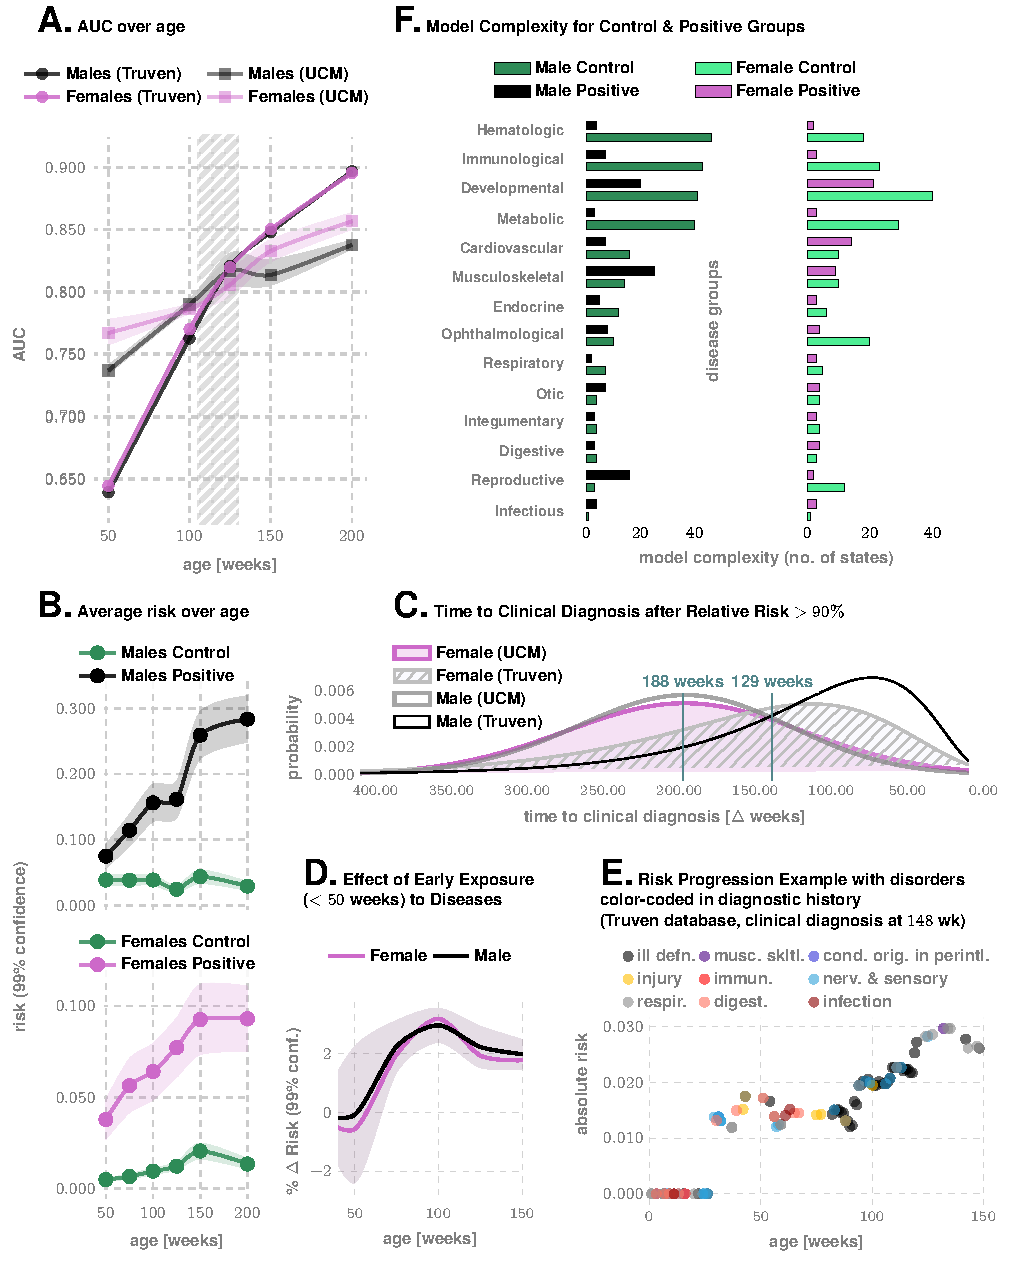
\includegraphics[width=0.85\textwidth]{Figures/External/perfB.pdf}
  \fi

  \captionN{\textbf{More details on Predictive Performance and Variation of Inferred Risk.} Panel A illustrates AUC achieved as a function of
    patient age, for the Truven and UCM datasets. The shaded area outlines the 2 - 2.5  years of age, and  shows that we achieve $>80\%$ AUC for either sex from shortly after 2 years.   Panel B illustrates how the average risk changes with time for the control and the positive cohorts. Panel C shows the distribution of the prediction horizon: the time to a clinical diagnosis after inferred  relative risk crosses $90\%$. Panel D shows that for each new disease code for a low-risk child, ASD risk increases by approximately $2\%$ for either sex. Panel E illustrates the risk progression of a specific, ultimately autistic male child in the Truven database. Abbreviations in the legend: ill defn. (Symptoms, Signs, And Ill-Defined Conditions),   musc. skltl. (Diseases Of The Musculoskeletal System And Connective Tissue), cond. orig. in perintl. (Certain Conditions Originating In The Perinatal Period), immun. (Endocrine, Nutritional And Metabolic Diseases, And Immunity Disorders), nerv. \& sensory (Diseases Of The Nervous System And Sense Organs), respir. (Respiratory Disorders), and digest. (Digestive Disorders). Panel F illustrates  how inferred models differ between the control vs. the \treatment cohorts. On average, models get less complex, implying the exposures get more statistically independent.}\label{fig2}
\end{figure*}
\else
\refstepcounter{figure}\label{fig2}
\fi
% ###########################################################
% ###########################################################
% ###########################################################
\ifFIGS
% ###########################################################
\begin{figure}[!ht]
  \tikzexternalenable
  \tikzsetnextfilename{perfCv}

  \centering
  
  \def\AXISCOL{white}
  \def\TEXTCOL{gray}
  \iftikzX
  \input{Figures/figprcv_.tex}
  \else
  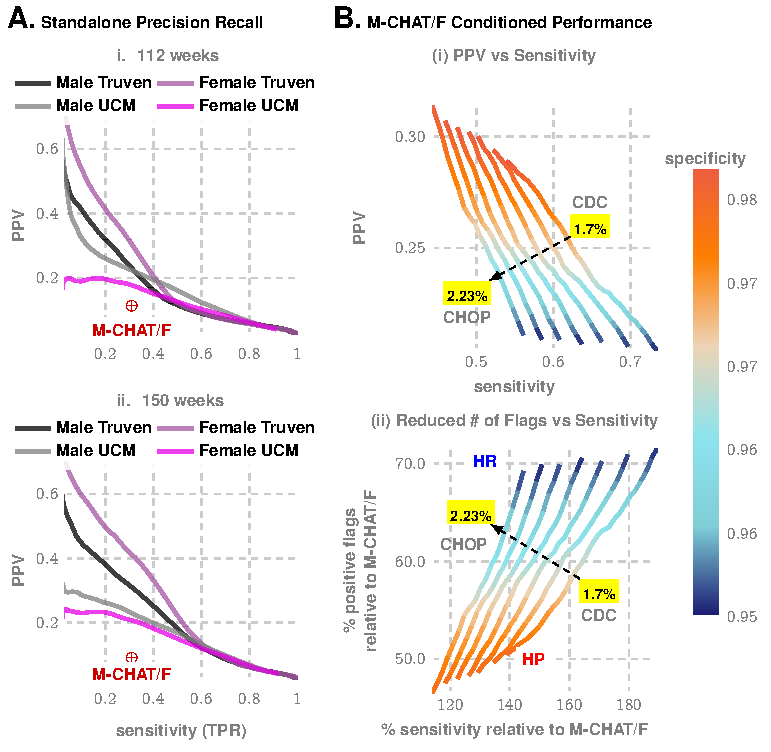
\includegraphics[width=0.5\textwidth]{Figures/External/perfCv.pdf}
  \fi

  \captionN{\textbf{Metrics relevant to clinical practice: PPV vs Sensitivity trade-offs.} Panel A shows the precision/recall curves, $i.e.$,  the trade-off between PPV and sensitivity. Panel B shows how we can boost performance using population stratification from the distribution of M-CHAT/F scores in the population, as reported by the CHOP study~\cite{pmid31562252}. Panel C illustrates the boosted performance compared to M-CHAT/F alone,
    measured by the relative percentage increase in sensitivity, and percentage decrease in positive screens. Note that the population prevalence impacts this optimization, and hence  we have  a distinct  curve for each prevalence value ($1.7\%$ is the CDC estimate, while $2.23\%$ is reported by the CHOP study).  The two extreme operating zones marked as High Precision (HP) and High Recall (HR): if we choose to operate in HR, then we do not reduce the number of positive screens by much, but maximize sensitivity, while by operating in HP, we do not increase sensitivity by much but double the PPV achieved in current practice. Note in all these zones, we maintain specificity above $95\%$, which is the current state of art, implying that by doubling the PPV, we can halve the number of positive screens currently reported, thus potentially sharply reducing the queues and wait-times. }\label{figprc}
\end{figure}

% ###########################################################
\else
\refstepcounter{figure}\label{figprc}
\fi 
% ###########################################################
% ##########################################
% ####################################
\def\RCOL{\rowcolor{teal!40}}
%#################################### 
\begin{table*}[t]   
\centering 
\captionN{PPV Achieved at 100, 112 and 150 Weeks For Each Dataset and Gender {\bf (M-CHAT/F:  sensitivity=$38.8\%$, specificity=$95\%$, PPV=$14.6\%$ between 16 and  26 months ($\approx$112 weeks))}}\label{EXT-tabssp}

  \vskip .5em

\begin{tabular}{L{.75in}|L{.75in}|L{.75in}|L{.5in}|L{.5in}|L{.75in}}
\hline
weeks&specificity&sensitivity&PPV&gender&dataset\\\hline
100&0.92&0.39&0.14&F&UCM\\\hline
100&0.95&0.39&0.19&M&UCM\\\hline
100&0.93&0.39&0.13&F&Truven\\\hline
100&0.91&0.39&0.10&M&Truven\\\hline
%\RCOL 112&0.94&0.35&0.17&F&UCM\\\hline
\RCOL 112&0.93&0.39&0.16&F&UCM\\\hline
\RCOL 112&0.95&0.39&0.20&M&UCM\\\hline
\RCOL 112&0.96&0.39&0.22&F&Truven\\\hline
\RCOL 112&0.95&0.39&0.17&M&Truven\\\hline
150&0.94&0.39&0.19&F&UCM\\\hline
150&0.98&0.39&0.34&F&Truven\\\hline
150&0.97&0.39&0.26&M&Truven\\\hline
150&0.97&0.39&0.26&M&UCM\\\hline

\end{tabular}
\end{table*}  
%####################################
% %####################################

%#################################### 
\begin{table*}[t]
\centering
\captionN{Personalized Operation Conditioned on M-CHAT/F Scores at  26 months}\label{EXT-tabboost}
  \vskip .5em

\begin{tabular} {L{.33in}|L{.33in}|L{.33in}|L{.33in}||L{.35in}|L{.35in}|L{.375in}||L{.375in}|L{.35in}|L{.35in}||L{.6in}}
\hline
\multicolumn{4}{c||}{\cellcolor{lightgray!60}M-CHAT/F Outcome}  & \multicolumn{3}{c||}{\mnp{.9in}{\vskip .2em global performance (Truven)\vskip .2em  } }&\multicolumn{3}{c||}{\mnp{1in}{\vskip .2em global performance\\(UCM)\vskip .2em }} &  \multirow{3}{*}{prevalence$^\star$}\\\cline{0-9}
 0-2  NEG & 3-7  NEG & 3-7  POS & $\geq  8$  POS & \multirow{2}{*}{\mnp{.1in}{speci-ficity}} & \multirow{2}{*}{\mnp{.1in}{sensi-tivity}} &\multirow{2}{*}{PPV}& \multirow{2}{*}{\mnp{.1in}{speci-ficity}} & \multirow{2}{*}{\mnp{.1in}{sensi-tivity}} & \multirow{2}{*}{PPV} & \\\cline{0-3}
\multicolumn{4}{c}{\cellcolor{lightgray} specificity choices}  & & & &&&&\\\hline 
  0.2&0.54&0.83&0.98&0.95&0.585&0.209&0.95&0.505&0.186&0.022\\\hline 
0.21&0.53&0.83&0.98&0.95&0.586&0.208&0.95&0.506&0.184&0.022\\\hline 
0.42&0.87&0.98&0.99&0.98&0.433&0.331&0.98&0.347&0.284&0.022\\\hline 
0.48&0.87&0.97&0.99&0.98&0.432&0.331&0.98&0.355&0.289&0.022\\\hline 
0.38&0.54&0.94&0.98&0.95&0.736&0.203&0.95&0.628&0.178&0.017\\\hline 
0.3&0.55&0.94&0.98&0.95&0.737&0.203&0.95&0.633&0.179&0.017\\\hline 
0.58&0.96&0.98&0.99&0.98&0.492&0.302&0.98&0.373&0.247&0.017\\\hline 
0.59&0.96&0.98&0.99&0.98&0.491&0.303&0.98&0.372&0.248&0.017\\\hline 
0.46&0.92&0.97&0.99&0.977&0.534&0.291&0.977&0.448&0.256&0.017\\\hline 
0.48&0.92&0.97&0.99&0.978&0.533&0.292&0.978&0.448&0.257&0.017\\\hline 
 
\end{tabular}
\vskip 1em

\flushleft
$^\star$Prevalence reported by CDC is $1.7\%$, while the CHOP study reports a value of $2.23\%$. The results of our optimization depend on the prevalence estimate.
\end{table*}  
%####################################
%###########################################################
%###########################################################
\ifFIGS
\begin{figure*}[!t]
  \tikzexternalenable
    \tikzsetnextfilename{comorbidA}

\def\DATA{../../data_latest}
\iftikzX
 

\pgfplotsset{
    discard if/.style 2 args={
        x filter/.code={
            \edef\tempa{\thisrow{#1}}
            \edef\tempb{#2}
            \ifx\tempa\tempb
                \def\pgfmathresult{inf}
            \fi
        }
    },
    discard if not/.style 2 args={
        x filter/.code={
            \edef\tempa{\thisrow{#1}}
            \edef\tempb{#2}
            \ifx\tempa\tempb
            \else
                \def\pgfmathresult{inf}
            \fi
        }
    }
  }

  \begin{tikzpicture}[font=\bf\sffamily\fontsize{8}{10}\selectfont]
  \def\TEXTCOL{gray}
  \tikzset{
    hatch distance/.store in=\hatchdistance,
    hatch distance=20pt,
    hatch thickness/.store in=\hatchthickness,
    hatch thickness=2pt
  }


\pgfplotsset{
    accommodate labels/.code 2 args={
        \newlength{\myl}
        \pgfplotstableread{#1}\data
        \def\largestlength{0}
        \pgfplotstableforeachcolumnelement{#2}\of\data\as\cell{
            \settowidth{\myl}{\pgfinterruptpicture\cell\endpgfinterruptpicture}
            \pgfmathsetmacro\largestlength{max(\the\myl,\largestlength)}
        }
        \pgfplotsset{
            enlarge x limits={
                upper,              value=1/(1-(\largestlength+4pt)/\pgfkeysvalueof{/pgfplots/width})-1
            }
        }
    }
}

\def\COLDR{white}
\definecolor{alizarin}{rgb}{0.82, 0.1, 0.26}
\definecolor{amber}{rgb}{1.0, 0.75, 0.0}
\definecolor{amethyst}{rgb}{0.6, 0.4, 0.8}
\definecolor{apricot}{rgb}{0.98, 0.81, 0.69}
\definecolor{atomictangerine}{rgb}{1.0, 0.6, 0.4}
\definecolor{awesome}{rgb}{1.0, 0.13, 0.32}
\definecolor{azurec}{rgb}{0.0, 0.5, 1.0}
\definecolor{ballblue}{rgb}{0.13, 0.67, 0.8}
\definecolor{bittersweet}{rgb}{1.0, 0.44, 0.37}
\definecolor{bluem}{rgb}{0.0, 0.5, 0.69}
\definecolor{brightturquoise}{rgb}{0.03, 0.91, 0.87}
\definecolor{fiveA}{HTML}{30a2da}
\definecolor{fiveB}{HTML}{fc4f30}
\definecolor{fiveC}{HTML}{e5ae38}
\definecolor{fiveD}{HTML}{6d904f}
\definecolor{fiveE}{HTML}{8b8b8b}



\def\COLBA{Red4}
\def\COLBB{alizarin}
\def\COLBI{Red1}
\def\COLBG{MediumBlue!70}
\def\COLBC{lightgray}
\def\COLBD{Green2}
\def\COLBE{fiveE}
\def\COLBF{SeaGreen3}
\def\COLBH{Cyan3}
\def\COLBJ{bittersweet}
\def\COLBK{Orchid3}
\def\COLBL{black}
\def\COLDM{amber}
\def\COLML{DarkGreen!90}
\def\COLPA{Orchid4}

\def\CINF{Red4}
\def\CNEO{SeaGreen4}
\def\CIMM{Red1}
\def\CBLD{lightgray}
\def\CNRV{fiveA}
\def\CCIR{Green2}
\def\CRSP{fiveE}
\def\CDIG{bittersweet}
\def\CSKN{Cyan3}
\def\CMSK{Indigo}
\def\CCNT{Orchid3}
\def\CPRI{MediumBlue!80}
\def\CINJ{amber}
\def\CMNT{DarkGreen!90}
\def\CGNT{DarkOrange3}
\def\CILL{black}
\def\HCOL{black}
\def\HBLK{gray}


  
  % \makeatletter
  % \pgfdeclarepatternformonly[\hatchdistance,\hatchthickness]{flexible hatch}
  % {\pgfqpoint{0pt}{0pt}}
  % {\pgfqpoint{\hatchdistance}{\hatchdistance}}
  % {\pgfpoint{\hatchdistance-1pt}{\hatchdistance-1pt}}%
  % {
  %   \pgfsetcolor{\tikz@pattern@color}
  %   \pgfsetlinewidth{\hatchthickness}
  %   \pgfpathmoveto{\pgfqpoint{0pt}{0pt}}
  %   \pgfpathlineto{\pgfqpoint{\hatchdistance}{\hatchdistance}}
  %   \pgfusepath{stroke}
  % }
  % \makeatother
  % \pgfdeclarepatternformonly{north east lines wide}%
  % {\pgfqpoint{-1pt}{-1pt}}%
  % {\pgfqpoint{10pt}{10pt}}%
  % {\pgfqpoint{9pt}{9pt}}%
  % {
  %   \pgfsetlinewidth{0.4pt}
  %   \pgfpathmoveto{\pgfqpoint{0pt}{0pt}}
  %   \pgfpathlineto{\pgfqpoint{9.1pt}{9.1pt}}
  %   \pgfusepath{stroke}
  % }


  \def\COMPA{\DATA/figfiles/age_3_mf_logodds_s_Mcodes.csv}
  \def\COMPB{\DATA/figfiles/age_3_mf_logodds_s_Fcodes.csv}
  \def\COMPA{Figures/NEWMcodes.csv}
  \def\COMPB{Figures/NEWFcodes.csv}
  \def\COMPMF{\DATA/figfiles/mf_logodds_c_MFComp.csv}
  \def\COMPMFA{\DATA/figfiles/age_3_mf_logodds_c_MFComp.csv}
  \def\COMPMF{Figures/NEW1YRMFComp.csv}
  \def\COMPMFA{Figures/NEWMFComp.csv}
  
  \def\WDTXX{1.85in}
  \def\WDTX{1.75in}
  \def\WDTXC{1.95in}
  \def\HGTX{6.85in} 
  \def\HGTXB{6.85in}
  \def\HGTXC{4in}
  \def\OPC{.9}
  \def\BWIDTH{7.5pt}
  \def\BWIDTHB{8pt}
  \def\BWIDTHC{6pt} 
  \def\BWIDTHD{5pt}


  

\clip (.8in,0.25in) rectangle (7.8in,-9.25in);

  
    \node [anchor=north west,align=left] (A) at (0,0) {
        \begin{tikzpicture}[text=\TEXTCOL]
%
 %  \def\basis{1}
%   \pgfplotsset
%   {
%     x coord trafo/.code={\pgfmathparse{symlog(#1,\basis)}\pgfmathresult},
%     x coord inv trafo/.code={\pgfmathparse{symexp(#1,\basis)}\pgfmathresult},
%     xticklabel style={/pgf/number format/.cd,int detect,precision=2},
% }


          \begin{axis}[legend style={anchor=east,at={(0.5,1.05)},inner sep=3pt,draw=none,fill=white,fill opacity=.850,align=right,text opacity=1,font=\bf\sffamily\fontsize{8}{9}\selectfont},axis line style={lightgray, opacity=0, thin},%
        enlargelimits=false,
        anchor=north west,
        height=\HGTX,
        width=\WDTXX,
        % xbar,
        ytick=data,% crucial line for the xticklabels directive 
        xmin=3.925,
        %xmax=2000,
        %accommodate labels={\DISX}{description},
        yticklabels from table={\COMPA}{code},
        yticklabel style
        ={font=\bf\sffamily\fontsize{7}{7}\selectfont,
          align=right,rotate=0, text width=1.1in,
          anchor=east, yshift=0in,xshift=-.0450in,text=\TEXTCOL},
        major tick length=0pt,,text opacity=1,
        %xticklabel style=
        %{font=\bf\sffamily\fontsize{7}{7}\selectfont,
        %  text=\TEXTCOL},
        %grid,
        grid style={lightgray, dashed,opacity=.70},
        axis on top=false, bar width=\BWIDTH,
        xlabel={log odds ratio of normalized prevalence},
        scaled x ticks=false,
        xlabel style={yshift=0.05in,text=\TEXTCOL,text opacity=1},
        ylabel style={xshift=-.25in,yshift=0.075in,text=\TEXTCOL,text opacity=1},
        enlarge y limits=.0150,
         x tick label style={/pgf/number format/fixed,/pgf/number format/precision=2,/pgf/number format/fixed zerofill,
     /pgf/number format/1000 sep = %\thinspace % Optional if you want to replace comma as the 1000 separator 
   },
   nodes near coords,,visualization depends on=x \as \rawx,
    every node near coord/.append style={anchor=west,align=left, text width=2in,font=\sffamily\rm\fontsize{8}{8}\selectfont,text=darkgray,text opacity=1,
        shift={(axis direction cs:0.01*\rawx,0)}},
   point meta=explicit symbolic,ylabel={},
   , %xtick ={-0.03,0,0.03},
  % xmax=0.03,xmin=-0.03,
        ] 

        \addplot[draw=none,fill=none,xbar,area legend,opacity=\OPC,text opacity=\OPC] table [ 
        y expr=\coordindex,
        x=pn,meta=description
        ] {\COMPA};

        \def\DISMM{\COMPA}
        
          \addplot[draw=\CINF,fill=\CINF,xbar,area legend,opacity=\OPC,text opacity=\OPC] table [ 
        y expr=\coordindex,
        x=pn, discard if not={icdclass}{0.0}
        ] {\DISMM};
          \addplot[draw=\CNEO,fill=\CNEO,xbar,area legend,opacity=\OPC,text opacity=\OPC] table [ 
        y expr=\coordindex,
        x=pn, discard if not={icdclass}{1.0}
        ] {\DISMM};
        \addplot[draw=\CIMM,fill=\CIMM,xbar,area legend,opacity=\OPC,text opacity=\OPC] table [ 
        y expr=\coordindex,
        x=pn, discard if not={icdclass}{2.0}
        ] {\DISMM};
        \addplot[draw=\CBLD,fill=\CBLD,xbar,area legend,opacity=\OPC,text opacity=\OPC] table [ 
        y expr=\coordindex,
        x=pn, discard if not={icdclass}{3.0}
        ] {\DISMM};
        \addplot[draw=\CMNT,fill=\CMNT,xbar,area legend,opacity=\OPC,text opacity=\OPC] table [ 
        y expr=\coordindex,
        x=pn, discard if not={icdclass}{4.0}
        ] {\DISMM};
        \addplot[draw=\CNRV,fill=\CNRV,xbar,area legend,opacity=\OPC,text opacity=\OPC] table [ 
        y expr=\coordindex,
        x=pn, discard if not={icdclass}{5.0}
        ] {\DISMM};
        \addplot[draw=\CCIR,fill=\CCIR,xbar,area legend,opacity=\OPC,text opacity=\OPC] table [ 
        y expr=\coordindex,
        x=pn, discard if not={icdclass}{6.0}
        ] {\DISMM};
        \addplot[draw=\CRSP,fill=\CRSP,xbar,area legend,opacity=\OPC,text opacity=\OPC] table [ 
        y expr=\coordindex,
        x=pn, discard if not={icdclass}{7.0}
        ] {\DISMM};
        \addplot[draw=\CDIG,fill=\CDIG,xbar,area legend,opacity=\OPC,text opacity=\OPC] table [ 
        y expr=\coordindex,
        x=pn, discard if not={icdclass}{8.0}
        ] {\DISMM};
        \addplot[draw=\CGNT,fill=\CGNT,xbar,area legend,opacity=\OPC,text opacity=\OPC] table [ 
        y expr=\coordindex,
        x=pn, discard if not={icdclass}{9.0}
        ] {\DISMM};
        \addplot[draw=\CSKN,fill=\CSKN,xbar,area legend,opacity=\OPC,text opacity=\OPC] table [ 
        y expr=\coordindex,
        x=pn, discard if not={icdclass}{11.0}
        ] {\DISMM};
        \addplot[draw=\CMSK,fill=\CMSK,xbar,area legend,opacity=\OPC,text opacity=\OPC] table [ 
        y expr=\coordindex,
        x=pn, discard if not={icdclass}{12.0}
        ] {\DISMM};
        \addplot[draw=\CCNT,fill=\CCNT,xbar,area legend,opacity=\OPC,text opacity=\OPC] table [ 
        y expr=\coordindex,
        x=pn, discard if not={icdclass}{13.0}
        ] {\DISMM};
        \addplot[draw=\CPRI,fill=\CPRI,xbar,area legend,opacity=\OPC,text opacity=\OPC] table [ 
        y expr=\coordindex,
        x=pn, discard if not={icdclass}{14.0}
        ] {\DISMM};
        \addplot[draw=\CILL,fill=\CILL,xbar,area legend,opacity=\OPC,text opacity=\OPC] table [ 
        y expr=\coordindex,
        x=pn, discard if not={icdclass}{15.0}
        ] {\DISMM};
        \addplot[draw=\CINJ,fill=\CINJ,xbar,area legend,opacity=\OPC,text opacity=\OPC] table [ 
        y expr=\coordindex,
        x=pn, discard if not={icdclass}{16.0}
        ] {\DISMM};
         
        
        % \addlegendentry{Female}
      \end{axis}
    \end{tikzpicture}};

      \node [anchor=south west,align=left] (B) at ([xshift=-1.65in]A.south east) {
        \begin{tikzpicture}[text=\TEXTCOL]
%
%   \def\basis{1}
%   \pgfplotsset
%   {
%     x coord trafo/.code={\pgfmathparse{symlog(#1,\basis)}\pgfmathresult},
%     x coord inv trafo/.code={\pgfmathparse{symexp(#1,\basis)}\pgfmathresult},
%     xticklabel style={/pgf/number format/.cd,int detect,precision=2},
% }


          \begin{axis}[legend style={anchor=east,at={(0.5,1.05)},inner sep=3pt,draw=none,fill=white,fill opacity=.85,align=right,text opacity=1,font=\bf\sffamily\fontsize{8}{9}\selectfont},axis line style={lightgray, opacity=0, thin},%
        enlargelimits=false,
        anchor=north west,
        height=\HGTXB,
        width=\WDTX,
        % xbar,
        ytick=data,% crucial line for the xticklabels directive 
        xmin=3.0,
        %xmax=2000,
        %accommodate labels={\DISX}{description},
        yticklabels from table={\COMPB}{code},
        yticklabel style
        ={font=\bf\sffamily\fontsize{7}{7}\selectfont,
          align=right,rotate=0, text width=1.1in,
          anchor=east, yshift=0in,xshift=-.0450in,text=\TEXTCOL},
        major tick length=0pt,,text opacity=1,
        %xticklabel style=
        %{font=\bf\sffamily\fontsize{7}{7}\selectfont,
        %  text=\TEXTCOL},
        %grid,
        grid style={lightgray, ultra thin,dashed,opacity=.7},
        axis on top=false, bar width=\BWIDTHB,
        xlabel={log odds ratio of normalized prevalence},
        scaled x ticks=false,
        xlabel style={yshift=0.05in,text=\TEXTCOL,text opacity=1},
        ylabel style={xshift=-.25in,yshift=0.1in,text=\TEXTCOL,text opacity=1},
        enlarge y limits=.015,
         x tick label style={/pgf/number format/fixed,/pgf/number format/precision=2,/pgf/number format/fixed zerofill,
     /pgf/number format/1000 sep = %\thinspace % Optional if you want to replace comma as the 1000 separator 
   },
   nodes near coords,,visualization depends on=x \as \rawx,
    every node near coord/.append style={anchor=west,align=left, text width=2in,font=\sffamily\rm\fontsize{8}{8}\selectfont,text=darkgray,text opacity=1,
        shift={(axis direction cs:0.01*\rawx,0.0)}},
   point meta=explicit symbolic,ylabel={ICD9 codes},
   , %xtick ={-0.03,0,0.03},
  % xmax=0.03,xmin=-0.03,
        ] 

        \addplot[draw=none,fill=none,xbar,area legend,opacity=\OPC,text opacity=\OPC] table [ 
        y expr=\coordindex,
        x=pn, meta=description
        ] {\COMPB};

        \def\DISMM{\COMPB}
        
          \addplot[draw=\CINF,fill=\CINF,xbar,area legend,opacity=\OPC,text opacity=\OPC] table [ 
        y expr=\coordindex,
        x=pn, discard if not={icdclass}{0.0}
        ] {\DISMM};
          \addplot[draw=\CNEO,fill=\CNEO,xbar,area legend,opacity=\OPC,text opacity=\OPC] table [ 
        y expr=\coordindex,
        x=pn, discard if not={icdclass}{1.0}
        ] {\DISMM};
        \addplot[draw=\CIMM,fill=\CIMM,xbar,area legend,opacity=\OPC,text opacity=\OPC] table [ 
        y expr=\coordindex,
        x=pn, discard if not={icdclass}{2.0}
        ] {\DISMM};
        \addplot[draw=\CBLD,fill=\CBLD,xbar,area legend,opacity=\OPC,text opacity=\OPC] table [ 
        y expr=\coordindex,
        x=pn, discard if not={icdclass}{3.0}
        ] {\DISMM};
        \addplot[draw=\CMNT,fill=\CMNT,xbar,area legend,opacity=\OPC,text opacity=\OPC] table [ 
        y expr=\coordindex,
        x=pn, discard if not={icdclass}{4.0}
        ] {\DISMM};
        \addplot[draw=\CNRV,fill=\CNRV,xbar,area legend,opacity=\OPC,text opacity=\OPC] table [ 
        y expr=\coordindex,
        x=pn, discard if not={icdclass}{5.0}
        ] {\DISMM};
        \addplot[draw=\CCIR,fill=\CCIR,xbar,area legend,opacity=\OPC,text opacity=\OPC] table [ 
        y expr=\coordindex,
        x=pn, discard if not={icdclass}{6.0}
        ] {\DISMM};
        \addplot[draw=\CRSP,fill=\CRSP,xbar,area legend,opacity=\OPC,text opacity=\OPC] table [ 
        y expr=\coordindex,
        x=pn, discard if not={icdclass}{7.0}
        ] {\DISMM};
        \addplot[draw=\CDIG,fill=\CDIG,xbar,area legend,opacity=\OPC,text opacity=\OPC] table [ 
        y expr=\coordindex,
        x=pn, discard if not={icdclass}{8.0}
        ] {\DISMM};
        \addplot[draw=\CGNT,fill=\CGNT,xbar,area legend,opacity=\OPC,text opacity=\OPC] table [ 
        y expr=\coordindex,
        x=pn, discard if not={icdclass}{9.0}
        ] {\DISMM};
        \addplot[draw=\CSKN,fill=\CSKN,xbar,area legend,opacity=\OPC,text opacity=\OPC] table [ 
        y expr=\coordindex,
        x=pn, discard if not={icdclass}{11.0}
        ] {\DISMM};
        \addplot[draw=\CMSK,fill=\CMSK,xbar,area legend,opacity=\OPC,text opacity=\OPC] table [ 
        y expr=\coordindex,
        x=pn, discard if not={icdclass}{12.0}
        ] {\DISMM};
        \addplot[draw=\CCNT,fill=\CCNT,xbar,area legend,opacity=\OPC,text opacity=\OPC] table [ 
        y expr=\coordindex,
        x=pn, discard if not={icdclass}{13.0}
        ] {\DISMM};
        \addplot[draw=\CPRI,fill=\CPRI,xbar,area legend,opacity=\OPC,text opacity=\OPC] table [ 
        y expr=\coordindex,
        x=pn, discard if not={icdclass}{14.0}
        ] {\DISMM};
        \addplot[draw=\CILL,fill=\CILL,xbar,area legend,opacity=\OPC,text opacity=\OPC] table [ 
        y expr=\coordindex,
        x=pn, discard if not={icdclass}{15.0}
        ] {\DISMM};
        \addplot[draw=\CINJ,fill=\CINJ,xbar,area legend,opacity=\OPC,text opacity=\OPC] table [ 
        y expr=\coordindex,
        x=pn, discard if not={icdclass}{16.0}
        ] {\DISMM};
         
        % \addlegendentry{Female}

        \draw [white,dashed,thick] (axis cs:4.00,-0.5) -- (axis cs:4.00,20.5) ;%node [midway,sloped,fill=gray,opacity=.3,text opacity=1,text=black] {4.00};
      \end{axis}
    \end{tikzpicture}};
   \node[fill=white,anchor=north west] (T) at ([xshift=-1.7in,yshift=0.225in]B.north east) {
      \arrayrulecolor{white}
      \setlength\arrayrulewidth{2pt}
      \mnp{2in}{\fontsize{7}{8}\selectfont\color{\TEXTCOL}
        {\large \color{black} ICD9 Class}
        \vskip 1em
        \begin{tabular}{L{.03in}L{1.5in}}
          \cellcolor{\CINF} & Infections \\\hline  %0
          \cellcolor{\CIMM} & Endocrine \& Immun. Dis.\\\hline %2
          %\cellcolor{\COLBI} & Skin \& subcut. tiss.\\\hline    %4
          \cellcolor{\CDIG} & Digestive Dis.\\\hline           %5
          %\cellcolor{\COLBC} & Mental Dis.\\\hline              %6
          \cellcolor{\CNRV} & Nervous Dis.\\\hline             %7
          \cellcolor{\CCIR} & Circulatory Dis.\\\hline         %8
          \cellcolor{\CRSP} & Respiratory Dis.\\\hline         %9
          \cellcolor{\CGNT} & Genitourinary Dis.\\\hline       %11
          \cellcolor{\CCNT} & Congenital Anomaly\\\hline       %13
          \cellcolor{\CPRI} & Cond. orig. in Perinatal Per.\\\hline %14
          \cellcolor{\CILL} & Ill-defined Cond. \& Symp. \\\hline   %15
          \cellcolor{\CMSK} & Musculosk. \& Conn. Tiss.\\\hline   %12
          \cellcolor{\CINJ} & Injury \& Poisoning   \\\hline %16
          \cellcolor{\CNEO} & Neoplasms    %1
          \end{tabular}
        }
      };


 \node [anchor=north west,align=left] (C) at ([yshift=-0.08in]A.south west) {
        \begin{tikzpicture}[text=\TEXTCOL]
%
%   \def\basis{1}
%   \pgfplotsset
%   {
%     x coord trafo/.code={\pgfmathparse{symlog(#1,\basis)}\pgfmathresult},
%     x coord inv trafo/.code={\pgfmathparse{symexp(#1,\basis)}\pgfmathresult},
%     xticklabel style={/pgf/number format/.cd,int detect,precision=2},
% }


          \begin{groupplot}[group style={group name=A,group size= 2 by 1,horizontal sep=0in,},legend style={anchor=east,at={(0.4,1.05)},inner sep=3pt,draw=none,fill=white,fill opacity=.85,align=right,text opacity=1,font=\bf\sffamily\fontsize{8}{9}\selectfont},axis line style={lightgray, opacity=0, thin},%
        enlargelimits=false,
        anchor=north west,
        height=2.6in,
        width=\WDTXC,
        % xbar,
        xlabel={log odds ratio of normalized prevalence},
   ]

   \nextgroupplot[   title={3 YR},  title style={yshift=-.1in},   ytick=data,% crucial line for the xticklabels directive 
       xmin=-2.50,
        %xmax=2000,
        %accommodate labels={\DISX}{description},
        yticklabels from table={\COMPMFA}{codedesc},
        yticklabel style
        ={font=\bf\sffamily\fontsize{7}{7}\selectfont,
          align=right,rotate=0, text width=4.1in,
          anchor=east, yshift=0in,xshift=-.0450in,text=\TEXTCOL},
        major tick length=0pt,,text opacity=1,
        %xticklabel style=
        %{font=\bf\sffamily\fontsize{7}{7}\selectfont,
        %  text=\TEXTCOL},
        grid,
        grid style={lightgray, dashed,opacity=.7},
        axis on top=false, bar width=\BWIDTHC,
        scaled x ticks=false,
        xlabel style={yshift=0.05in,text=\TEXTCOL,text opacity=1},
        ylabel style={xshift=-.25in,yshift=0.075in,text=\TEXTCOL,text opacity=1},
        enlarge y limits=.05,
        enlarge x limits=.05,
         x tick label style={/pgf/number format/fixed,/pgf/number format/precision=2,/pgf/number format/fixed zerofill,
     /pgf/number format/1000 sep = %\thinspace % Optional if you want to replace comma as the 1000 separator 
   },
   nodes near coords,,visualization depends on=x \as \rawx,
    every node near coord/.append style={anchor=west,align=left, text width=2in,font=\sffamily\rm\fontsize{8}{8}\selectfont,text=darkgray,text opacity=1,
        shift={(axis direction cs:0.01*\rawx,0.0)}},
   point meta=explicit symbolic,ylabel={},
   , %xtick ={-0.03,0,0.03},
  % xmax=0.03,xmin=-0.03,
]
   
        \addplot[draw=black,fill=\FXCOL,xbar,area legend,opacity=\OPC,text opacity=\OPC] table [ 
        y expr=\coordindex,
        x=pnF, %meta=codedesc
        ] {\COMPMFA};

        \def\DISMM{\COMPMFA}
        \def\PN{pnF}
        

        
        \def\OPC{.75}
        \def\PN{pnM}
        \addplot[draw=none,fill=none,xbar,bar width=\BWIDTHD,postaction={
         pattern=flexible hatch,
        hatch distance=5pt,
        hatch thickness=1pt,
        draw=none,
        pattern color=\HCOL, %ultra thick,
     },area legend,opacity=1,text opacity=\OPC] table [ 
        y expr=\coordindex,
        x=\PN, %meta=codedesc
        ] {\COMPMFA};


   \nextgroupplot[  title={5 YR},  title style={yshift=-.1in},  xlabel={},    ytick=data,% crucial line for the xticklabels directive 
       xmin=-2.5,xmax=4,
        %xmax=2000,
        %accommodate labels={\DISX}{description},
        yticklabels from table={\COMPMF}{codedesc},
        yticklabel style
        ={font=\bf\sffamily\fontsize{7}{7}\selectfont,
          align=right,rotate=0, text width=4.1in,
          anchor=east, yshift=0in,xshift=-.0450in,text=\TEXTCOL,text opacity=0},
        major tick length=0pt,,text opacity=1,
        %xticklabel style=
        %{font=\bf\sffamily\fontsize{7}{7}\selectfont,
        %  text=\TEXTCOL},
        grid,
        grid style={lightgray, dashed,opacity=.7},
        axis on top=false, bar width=\BWIDTHC,
        scaled x ticks=false,
        xlabel style={yshift=0.05in,text=\TEXTCOL,text opacity=1},
        ylabel style={xshift=-.25in,yshift=0.075in,text=\TEXTCOL,text opacity=1},
        enlarge y limits=.05,
        enlarge x limits=.05,
         x tick label style={/pgf/number format/fixed,/pgf/number format/precision=2,/pgf/number format/fixed zerofill,
           /pgf/number format/1000 sep = %\thinspace % Optional if you want to replace comma as the 1000 separator
           text opacity=1,
   },
   nodes near coords,,visualization depends on=x \as \rawx,
    every node near coord/.append style={anchor=west,align=left, text width=2in,font=\sffamily\rm\fontsize{8}{8}\selectfont,text=darkgray,text opacity=1,
        shift={(axis direction cs:0.01*\rawx,0.0)}},
   point meta=explicit symbolic,ylabel={},
   , %xtick ={-0.03,0,0.03},
  % xmax=0.03,xmin=-0.03,
]
   
        \addplot[draw=black,fill=\FXCOL,xbar,area legend,opacity=\OPC,text opacity=\OPC] table [ 
        y expr=\coordindex,
        x=pnF, %meta=codedesc
        ] {\COMPMF};

        \def\DISMM{\COMPMF}
        \def\PN{pnF}
        

        
        \def\OPC{.75}
        \def\PN{pnM}
        \addplot[draw=none,fill=none,xbar,bar width=\BWIDTHD,postaction={
         pattern=flexible hatch,
        hatch distance=5pt,
        hatch thickness=1pt,
        draw=none,
        pattern color=\HCOL, %ultra thick,
     },area legend,opacity=1,text opacity=\OPC] table [ 
        y expr=\coordindex,
        x=\PN, %meta=codedesc
        ] {\COMPMF};



        
      \end{groupplot}
    \end{tikzpicture}};


         \node[fill=white,anchor=north west,opacity=\OPC, fill opacity=1,,text=\TEXTCOL,text width=.15in,postaction={
         pattern=flexible hatch,
        hatch distance=5pt,
        hatch thickness=1pt,
        draw=none,
        pattern color=\HCOL, %ultra thick,
      },label={[,text=\TEXTCOL]0:Male}] (T) at ([xshift=-2.0in,yshift=-0.225in]C.north east) {};
         \node[draw=\HBLK,fill=\FXCOL,anchor=north west,opacity=\OPC, fill opacity=1,,text=\TEXTCOL,text width=.15in,label={[,text=\TEXTCOL]0:Female}] (T) at ([xshift=-2.0in,yshift=-0.4in]C.north east) {};
      
      
  \node[anchor=south west,align=left] (LA) at ([xshift=1in,yshift=0in]A.north west) {{\LARGE A.} Male (3 YR) };
  \node[anchor=south west,align=left] (LB) at ([xshift=3in,yshift=0in]$(LA.north west)!(B.north)!(LA.south west)$) {{\LARGE B.} Female (3 YR) };
   \node[anchor=south west,align=left] (LC) at ([yshift=-.25in]$(C.north west)!(LA.west)!(C.north east)$) {{\LARGE C.} Average Log Odds Ratios By Gender };
 
 % \node[anchor=south west,align=left] (LC) at ([xshift=1in,yshift=0.15in]R.north west) {{\LARGE C.} Codes with\\Maximum Mismatch Across Genders};
\end{tikzpicture}

 
 \else
  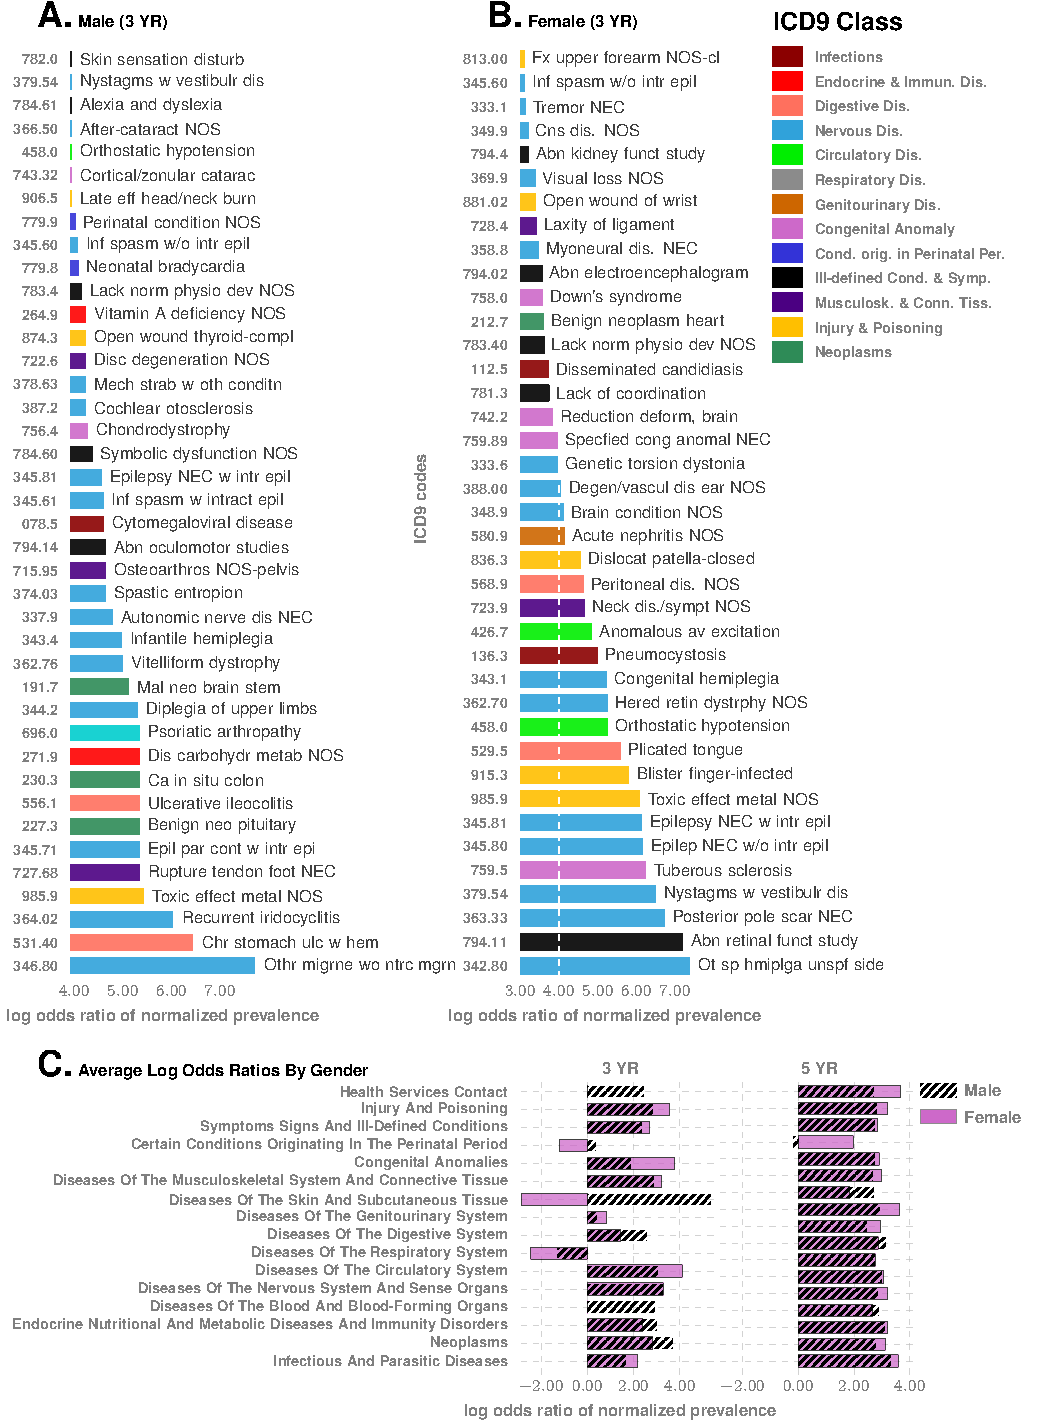
\includegraphics[width=0.9\textwidth]{Figures/External/comorbidA}
\fi
  \vspace{-5pt}
  
  \captionN{\textbf{Co-morbidity Patterns} Panel A and B. Difference in occurrence frequencies of diagnostic codes between true positive (TP) and true negative (TN) predictions. The dotted line on panel B shows the  abscissa lower cut-off in Panel A, illustrating the lower prevalence of codes in females. Panel C illustrates log-odds ratios for ICD9 disease categories at different ages. Importantly, the negative associations disappear when we consider older children, consistent with the lack of such reports in the literature which lack studies on very young cohorts. }\label{EXT-fig3}
  \vspace{-5pt}
  
\end{figure*}
\else
\refstepcounter{figure}\label{EXT-fig3}
\fi
% ###########################################################
% #############
